\documentclass[twoside,twocolumn]{article}
\usepackage{amsmath}
\usepackage{amssymb}
\usepackage[hmarginratio=1:1,top=32mm,columnsep=20pt]{geometry}
\usepackage[hang, small,labelfont=bf,up,textfont=it,up]{caption} 
\usepackage{booktabs}
\usepackage{enumitem}
\setlist[itemize]{noitemsep}
\usepackage{abstract}
\renewcommand{\abstractnamefont}{\normalfont\bfseries}
\renewcommand{\abstracttextfont}{\normalfont\small\itshape}
\usepackage{titlesec}
\renewcommand\thesection{\Roman{section}}
\renewcommand\thesubsection{\Alph{subsection}}
\renewcommand\thesubsubsection{\arabic{subsubsection}}
\titleformat{\section}[block]{\normalsize\bfseries\scshape\centering}{\thesection.}{1em}{}
\titleformat{\subsection}[block]{\normalsize\bfseries\centering}{\thesubsection.}{1em}{}
\titleformat{\subsubsection}[block]{\normalsize\centering}{\thesubsubsection.}{1em}{}
\usepackage{fancyhdr}
\pagestyle{fancy}
\fancyhead{}
\fancyhead[C]{Computational Physics Homework $\bullet$ May 2018 $\bullet$ Vol. I, No. 3}
\usepackage{titling}
\usepackage{hyperref}
\hypersetup{unicode}
\AtBeginShipoutFirst{\input{zhwinfonts.tex}}
\usepackage{bm}
\usepackage{braket}
\usepackage{CJKutf8}
\usepackage{xcolor}
\usepackage{dcolumn}
\usepackage{graphicx}
\usepackage{indentfirst}
\usepackage{listings}
\usepackage[toc, page, title, titletoc, header]{appendix}
\definecolor{grey}{rgb}{0.8,0.8,0.8}
\definecolor{darkgreen}{rgb}{0,0.3,0}
\definecolor{darkblue}{rgb}{0,0,0.3}
\def\lstbasicfont{\fontfamily{pcr}\selectfont\footnotesize}
\lstset{
	numbers=left,
	numberstyle=\small,
	showstringspaces=false,
	showspaces=false,
	tabsize=4,
	frame=single,
	basicstyle={\footnotesize\lstbasicfont},
	keywordstyle=\color{darkblue}\bfseries,
	identifierstyle=,
	commentstyle=\color{darkgreen},
	stringstyle=\color{black}
}
\lstloadlanguages{C,C++,Fortran,Java,Matlab,Mathematica,Python}
\setlength{\parindent}{2em}
\begin{document}
\begin{CJK*}{UTF8}{gkai}
%----------------------------------------------------------------------------------------
%	TITLE SECTION
%----------------------------------------------------------------------------------------

\setlength{\droptitle}{-4\baselineskip} % Move the title up
\pretitle{\begin{center}\Huge\bfseries} % Article title formatting
	\posttitle{\end{center}} % Article title closing formatting
\title{计算物理第三次作业} % Article title
\author{
	\textsc{梁旭民}\thanks{\noindent 指导老师:齐新老师} \\[1ex] % Your name
	\normalsize Cuiying Hornors College, Lanzhou University \\ % Your institution
	\normalsize \href{mailto:liangxm15@lzu.edu.cn}{liangxm15@lzu.edu.cn} % Your email address
}
\date{}
\renewcommand{\maketitlehookd}{
	\begin{abstract}
		本次计算物理作业主要通过打靶法求解边界为无穷高的线性势阱的一维schrodinger方程,并综合了前三章所有内容:Simpson积分、搜索法及弦切法求根、Numernov算法、打靶法。
	\end{abstract}
}
\maketitle

%----------------------------------------------------------------------------------------
%	SECTION 1
%----------------------------------------------------------------------------------------

\section{问题描述}
计算半导体硅中能谷电子在三角形势阱中的所有能量本征值和波函数,其中低能谷电子有效能量0.916$m_{e}$,势场宽度35nm,势阱深度1eV。(本征值无限接近连续时候根据自己程序精度舍弃)
\begin{figure}[h]
	\centering
	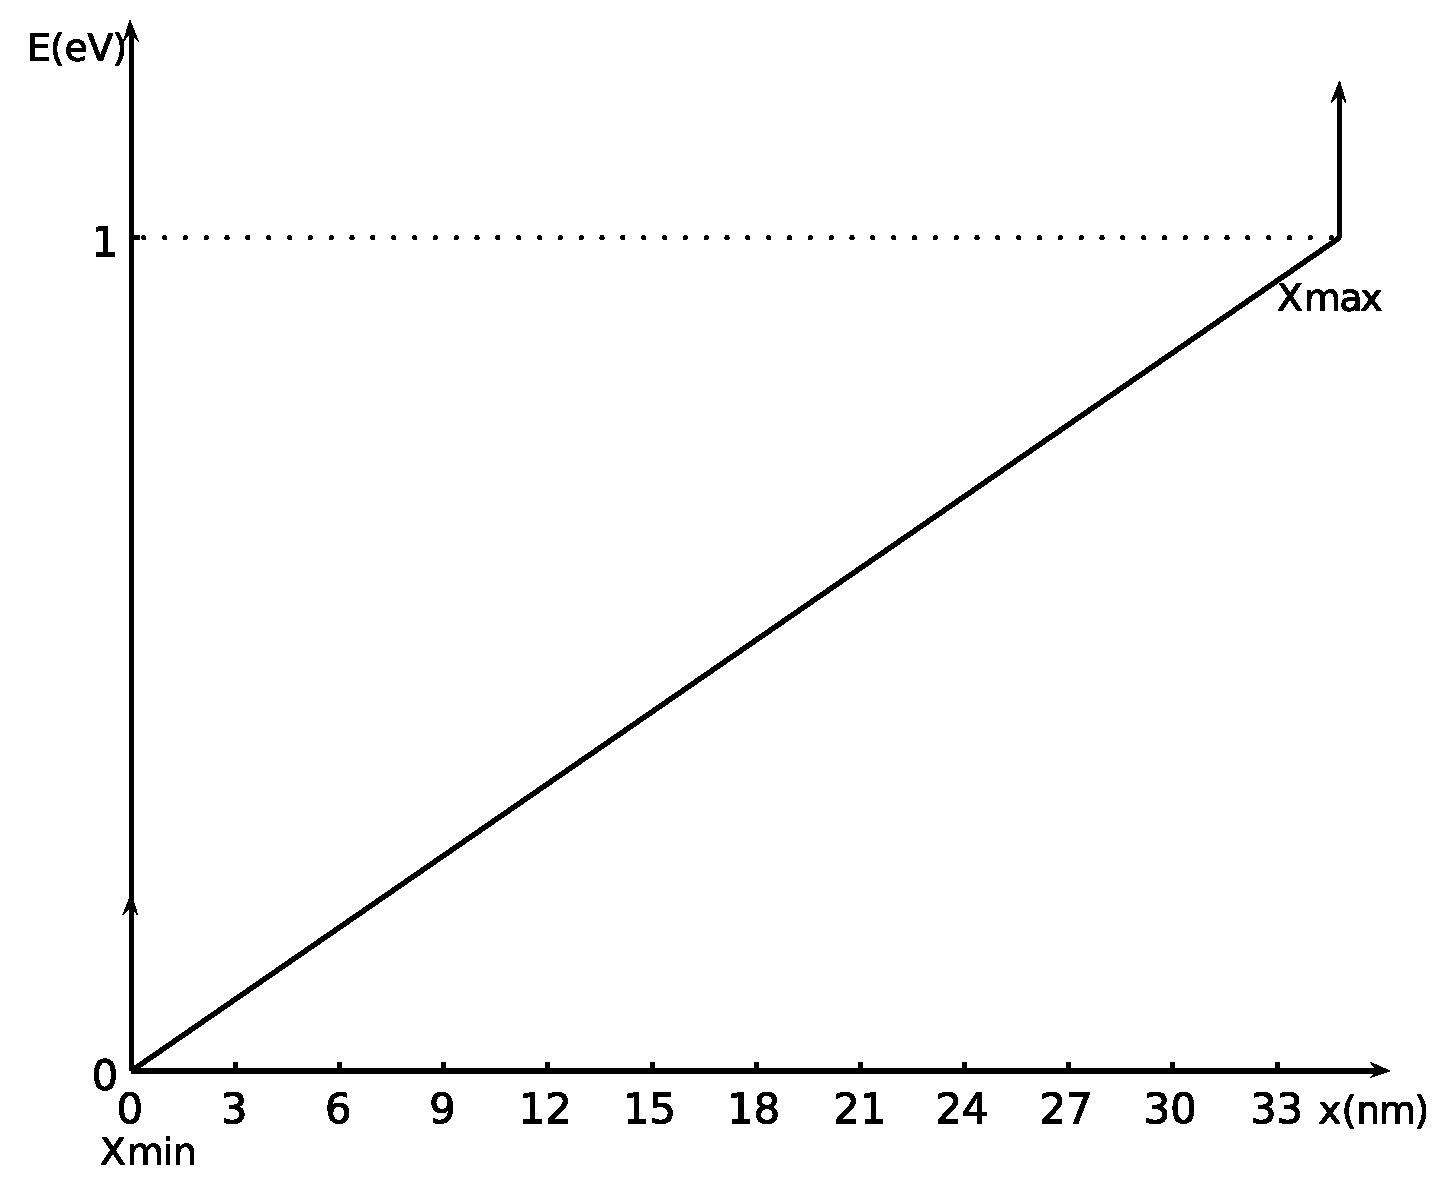
\includegraphics[width=0.9\linewidth]{./figure/fig1}
	\caption{一维位势V(x)图像(国际单位制下)}
	\label{fig:fig1}
\end{figure}

%----------------------------------------------------------------------------------------
%	SECTION 2
%----------------------------------------------------------------------------------------

\section{问题分析}
该问题本质上是求解定态schrodinger方程
\begin{equation*}
\left\{
\begin{aligned}
&\left[-\frac{d^{2}}{dx^{2}}+\frac{2m}{\hbar^{2}}(V(x)-E)\right]\psi(x)=0\\
&\psi(x_{min})=\psi(x_{max})=0
\end{aligned}
\right.
\end{equation*}
其中,势阱V(x)为
\begin{equation*}
\left\{
\begin{aligned}
&\frac{1}{35}x \qquad x<35nm\\
&\infty \quad\qquad x \geqslant 35nm
\end{aligned}
\right.
\end{equation*}

该本质问题相当于定解问题
\begin{equation*}
\left\{
\begin{aligned}
&\left(\frac{d^{2}}{dx^{2}}+k^{2}\right)\psi(x)=0\\
&\psi(x_{min})=\psi(x_{max})=0
\end{aligned}
\right.
\end{equation*}
本征值问题多了一个待定参数k,先猜测一个本征值k,设一个非零参数$\delta$,将该问题转化为初值问题
\begin{equation*}
\left\{
\begin{aligned}
&\left(\frac{d^{2}}{dx^{2}}+k^{2}\right)\psi(x)=0\\
&\psi(x_{min})=\psi(x_{max})=0\\
&\psi^{\prime}(x_{min})=\psi^{\prime}(x_{max})=\delta
\end{aligned}
\right.
\end{equation*}

%----------------------------------------------------------------------------------------
%	SECTION 3
%----------------------------------------------------------------------------------------

\section{Numerov算法简介}
Numerov方法属于四阶线性多步法,用于求解不出现一阶微分项的二阶常微分方程。Numerov方法属于隐式方法,但如果微分方程线性,则可转化为显式方法。该方法由 俄国天文学家Boris Vasil'evich Numerov提出。
\subsection{基本算法}
可由Numerov方法求解的微分方程形式为
\begin{equation*}
\left({\frac {d^{2}}{dx^{2}}}+f(x)\right)y(x)=0 
\end{equation*}
求出函数$y(x)$在区间$[a,b]$上等距格点上的值,从连续的两个格点上的函数值$x_{n-1}$和$x_{n}$开始,其他的函数值可由
\begin{equation*}
y_{n+1}={\frac {\left(2-{\frac {5h^{2}}{6}}f_{n}\right)y_{n}-\left(1+{\frac {h^{2}}{12}}f_{n-1}\right)y_{n-1}}{1+{\frac {h^{2}}{12}}f_{n+1}}}
\end{equation*}
算得。

其中,$f_{n}=f(x_{n})$和$y_{n}=y(x_{n})$为在格点$x_{n}$上的函数值,$h=x_{n}-x_{n-1}$为格点间距。

对于非线性方程,
\begin{equation*}
\frac{d^{2}}{dt^{2}}y=f(t,y)
\end{equation*}
则非线性方程的Numerov方法为
\begin{equation*}
y_{n+1}=2y_{n}-y_{n-1}+{\tfrac {1}{12}}h^{2}(f_{n+1}+10f_{n}+f_{n-1})
\end{equation*}

该式为隐式的线性多步方法。当$f$是$y$的线性函数时,该式变为显式方法,精度为4阶(Hairer,Nørsett \& Wanner 1993,§III.10)
\subsection{算法推导}
从$y(x_{n})$的Taylor展开开始, 我们可求$x_{n}$的相接邻点上的函数值
\begin{equation*}
\begin{aligned}
&y_{n+1}=y(x_{n}+h)=y(x_{n})+hy'(x_{n})+{\frac {h^{2}}{2!}}y''(x_{n}) \\
&+{\frac {h^{3}}{3!}}y'''(x_{n})+{\frac {h^{4}}{4!}}y''''(x_{n})+{\frac {h^{5}}{5!}}y'''''(x_{n})+{\mathcal {O}}(h^{6})\\
&y_{n-1}=y(x_{n}-h)=y(x_{n})-hy'(x_{n})+{\frac {h^{2}}{2!}}y''(x_{n})\\
&-{\frac {h^{3}}{3!}}y'''(x_{n})+{\frac {h^{4}}{4!}}y''''(x_{n})-{\frac {h^{5}}{5!}}y'''''(x_{n})+{\mathcal {O}}(h^{6}) 
\end{aligned}
\end{equation*}
上两式之和为
\begin{equation*}
y_{n-1}+y_{n+1}=2y_{n}+{h^{2}}y''_{n}+{\frac {h^{4}}{12}}y''''_{n}+{\mathcal {O}}(h^{6}) 
\end{equation*}
用所求微分方程的定义式$y''_{n}=-f_{n}y_{n}$替换掉$y''_{n}$
\begin{equation*}
h^{2}f_{n}y_{n}=2y_{n}-y_{n-1}-y_{n+1}+{\frac {h^{4}}{12}}y''''_{n}+{\mathcal {O}}(h^{6})
\end{equation*}
对所求微分方程的定义式$y''_{n}=-f_{n}y_{n}$取二次微分
\begin{equation*}
y''''(x)=-{\frac {d^{2}}{dx^{2}}}\left[f(x)y(x)\right]
\end{equation*}
将其代入到四阶微分项中,并把二阶导$\frac{d^{2}}{dx^{2}}\left[f(x)y(x)\right]$替换为$f_{n}y_{n}$的二阶差分公式$\frac {f_{n-1}y_{n-1}-2f_{n}y_{n}+f_{n+1}y_{n+1}}{h^{2}}$
\begin{equation*}
\begin{aligned}
&h^{2}f_{n}y_{n}=2y_{n}-y_{n-1}-y_{n+1}\\
&-{\frac {h^{4}}{12}}{\frac {f_{n-1}y_{n-1}-2f_{n}y_{n}+f_{n+1}y_{n+1}}{h^{2}}}+{\mathcal {O}}(h^{6})
\end{aligned}
\end{equation*}
求解$y_{n+1}$可得
\begin{equation*}
\begin{aligned}
&y_{n+1}={\frac {\left(2-{\frac {5h^{2}}{6}}f_{n}\right)y_{n}-\left(1+{\frac {h^{2}}{12}}f_{n-1}\right)y_{n-1}}{1+{\frac {h^{2}}{12}}f_{n+1}}}\\
&+{\mathcal {O}}(h^{6})
\end{aligned}
\end{equation*}
忽略掉$\mathcal{{O}}(h^{6})$就可以得到Numerov方法,最终收敛阶数为4(假定稳定)。
\subsection{算法应用}
在物理中用于数值求解任意势场中径向schrodinger方程:
\begin{equation*}
\left[-{\hbar ^{2} \over 2\mu }\left({\frac {1}{r}}{\partial ^{2} \over \partial r^{2}}r-{l(l+1) \over r^{2}}\right)+V(r)\right]R(r)=ER(r)
\end{equation*}
此式可重写为
\begin{equation*}
\left[{\partial ^{2} \over \partial r^{2}}-{l(l+1) \over r^{2}}+{2\mu \over \hbar ^{2}}\left(E-V(r)\right)\right]u(r)=0
\end{equation*}
其中$u(r)=rR(r)$与Numerov方法求解的方程形式做比较,则有
\begin{equation*}
f(x)={\frac {2\mu }{\hbar ^{2}}}\left(E-V(x)\right)-{\frac {l(l+1)}{x^{2}}}
\end{equation*}
这样,我们可以数值求解schrodinger方程。

%----------------------------------------------------------------------------------------
%	SECTION 4
%----------------------------------------------------------------------------------------

\section{算法设计}
选择打靶法求解该本征值问题。

从$x_{min}$出发积分,产生一个数值解$\psi_{<}$,它在经典禁戒的区指数增长,经过$x_{min}$进入经典允许的区域,并在此区域内振荡,但如果再经过$x_{max}$积分下去,会因为某个指数增长部分而使得数值不稳定。因此便需要将x分为两部分,并分别使用numerov算法积分求出波函数,对于中间的转折点则应该有条件
\begin{equation*}
\left\{
\begin{aligned}
&\psi_{<}=\psi_{>}\\
&\psi_{<}^{\prime}=\psi_{>}^{\prime}
\end{aligned}
\right.
\end{equation*}

因此,我们先通过给左右两部分的某一支数乘一个系数C使得
\begin{equation*}
\psi_{<}=\psi_{>}
\end{equation*}
并不断通过猜测的能量本征值,调节波函数光滑连续,将光滑作为判定条件即还需满足
\begin{equation*}
\psi_{<}^{\prime}=\psi_{>}^{\prime}
\end{equation*}

%----------------------------------------------------------------------------------------
%	SECTION 5
%----------------------------------------------------------------------------------------

\section{计算结果}
对于该问题,存在并求解出了36个能量本征值,从小到大依次为
\begin{equation*}
\begin{aligned}
&-9.229815 \quad&-8.676829 \quad&-8.227134 \\
&-7.819172 \quad&-7.439463 \quad&-7.083014 \\
&-6.746237 \quad&-6.426222 \quad&-6.120651 \\
&-5.827706 \quad&-5.545966 \quad&-5.011822 \\
&-4.757705 \quad&-4.511182 \quad&-4.271408 \\
&-4.037440 \quad&-3.808270 \quad&-3.582975 \\
&-3.360825 \quad&-3.141352 \quad&-2.709584 \\
&-2.497157 \quad&-2.287020 \quad&-2.079168 \\
&-1.873584 \quad&-1.670241 \quad&-1.469100 \\
&-1.270116 \quad&-1.073227 \quad&-0.878328 \\
&-0.685096 \quad&-0.492458 \quad&-0.297843 \\
&-0.097407 \quad&+0.112194 \quad
\end{aligned}
\end{equation*}

%----------------------------------------------------------------------------------------
%	SECTION 6
%----------------------------------------------------------------------------------------

\section{绘制波函数图像}
运用Python的openpyxl和pyplot库,通过循环读取工作簿不同工作表中的数据,分别绘制出对应与不同的能量本征值波函数图像
\begin{figure}[htb]
	\centering
	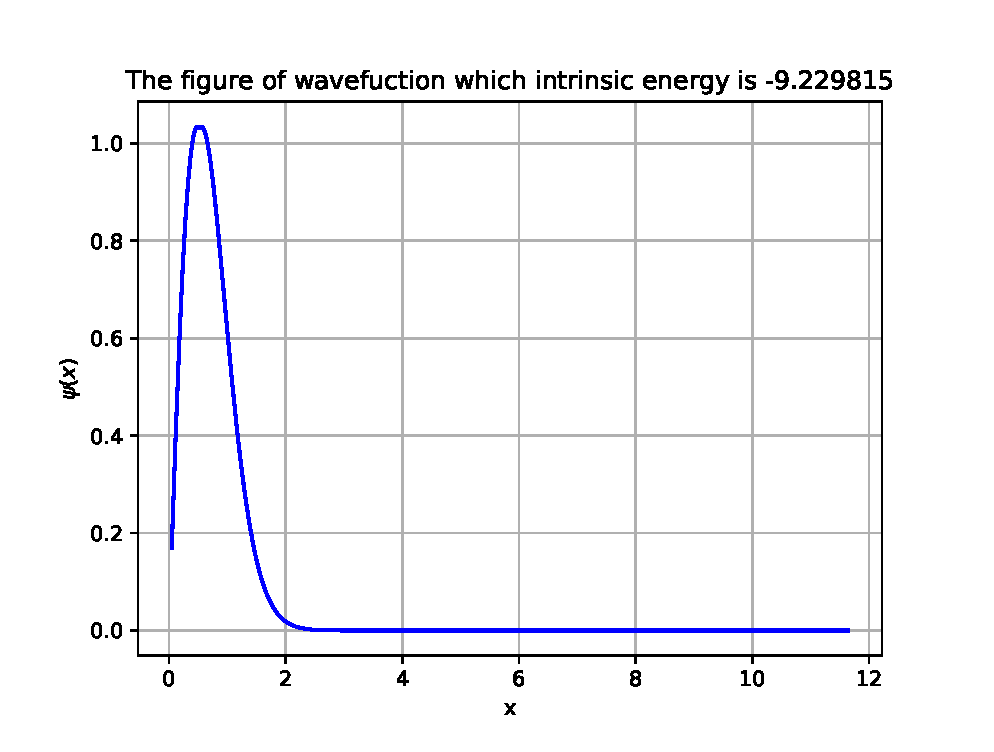
\includegraphics[width=0.98\linewidth]{figure/1}
	\label{fig:1}
\end{figure}
\begin{figure}[htb]
	\centering
	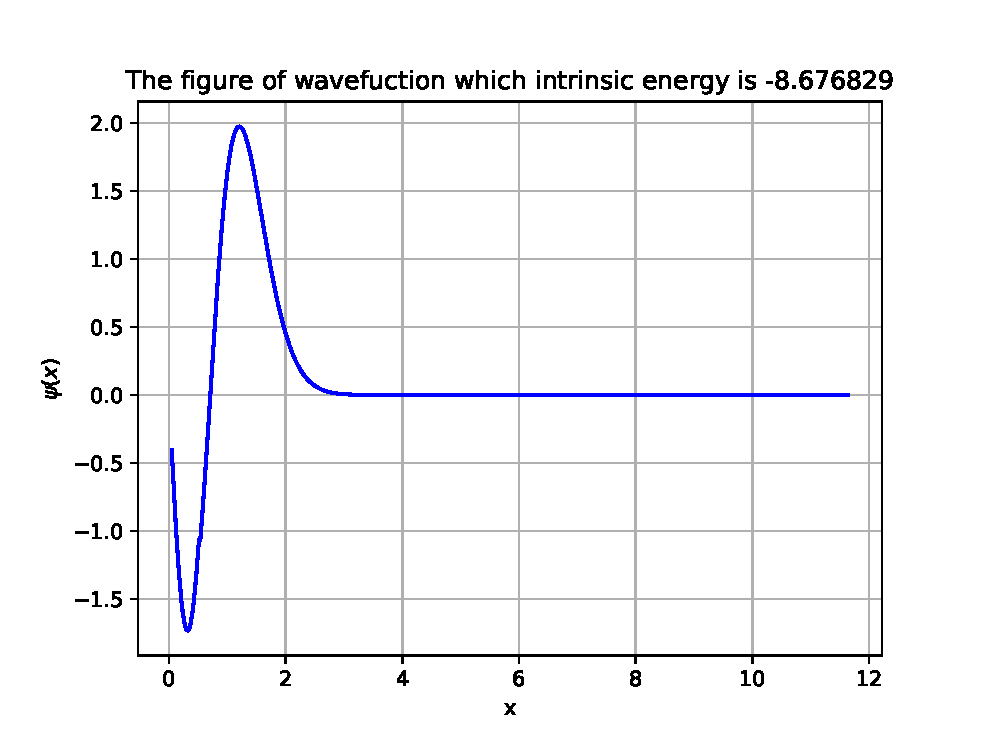
\includegraphics[width=0.98\linewidth]{figure/2}
	\label{fig:2}
\end{figure}
\begin{figure}[htb]
	\centering
	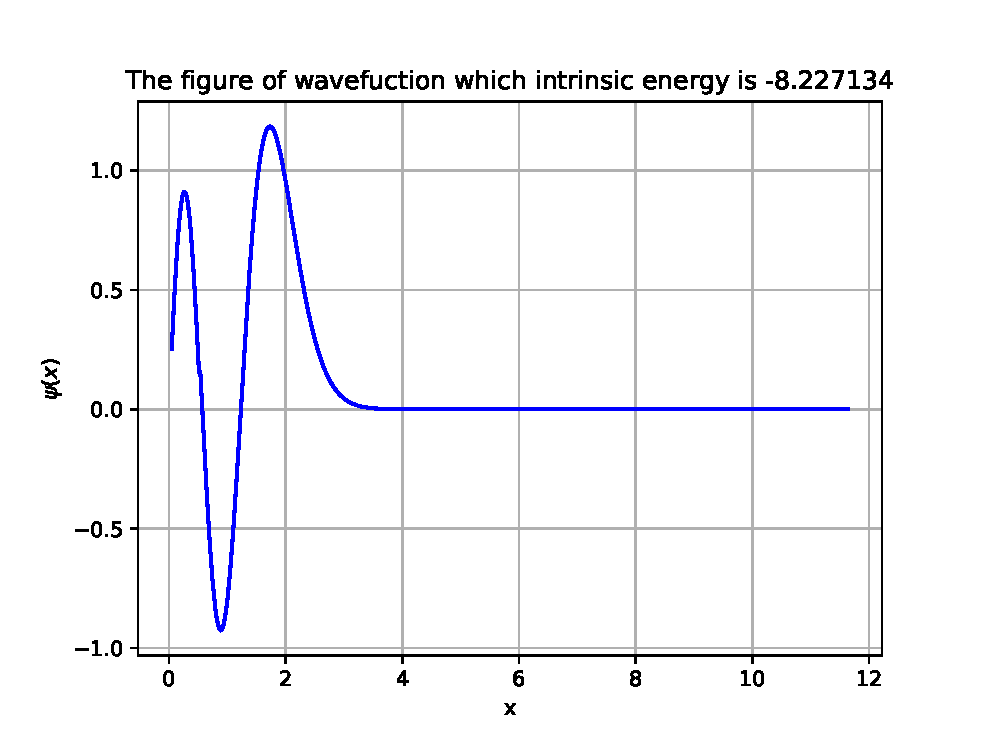
\includegraphics[width=0.98\linewidth]{figure/3}
	\label{fig:3}
\end{figure}
\begin{figure}[htb]
	\centering
	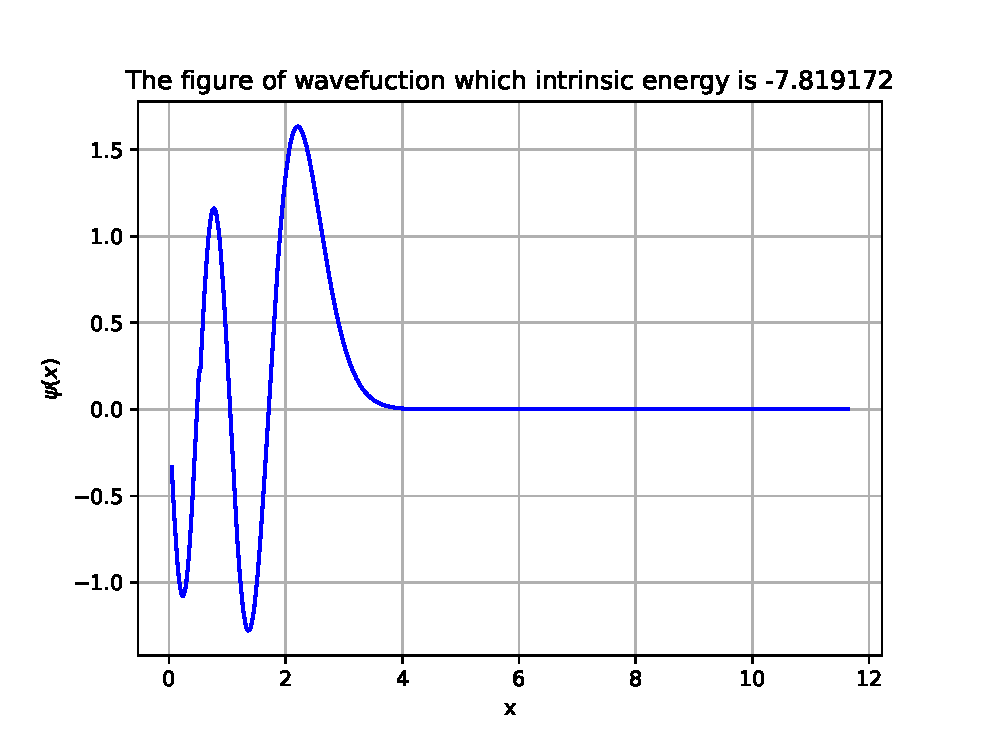
\includegraphics[width=0.98\linewidth]{figure/4}
	\label{fig:4}
\end{figure}

\newpage
\begin{figure}
	\centering
	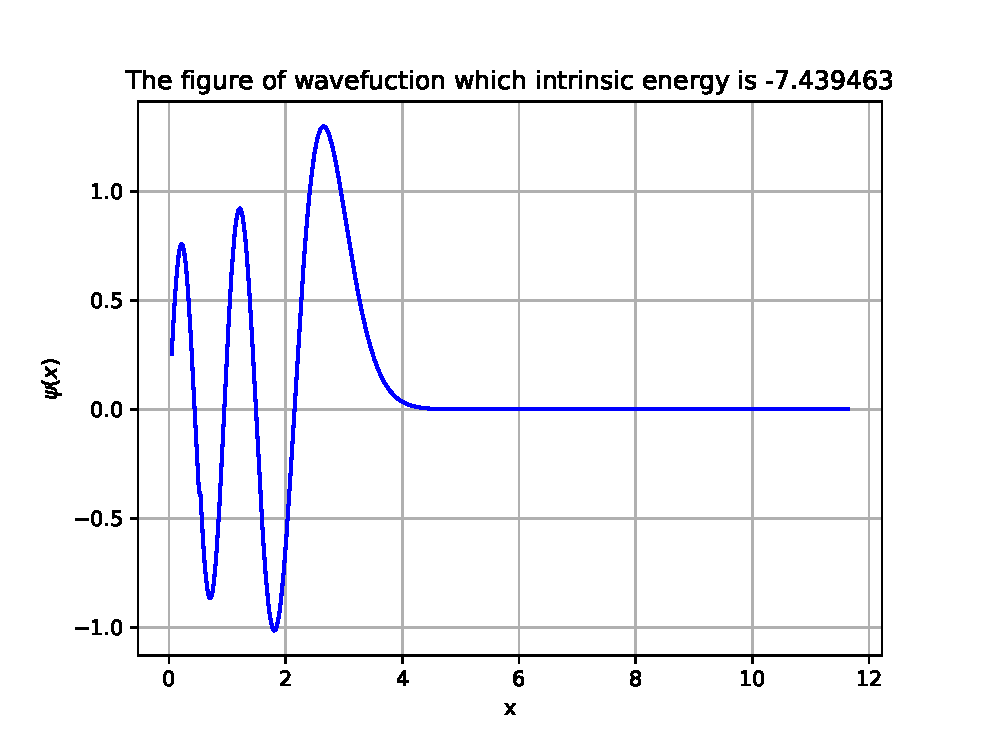
\includegraphics[width=0.9\linewidth]{figure/5}
	\label{fig:5}
\end{figure}
\begin{figure}
	\centering
	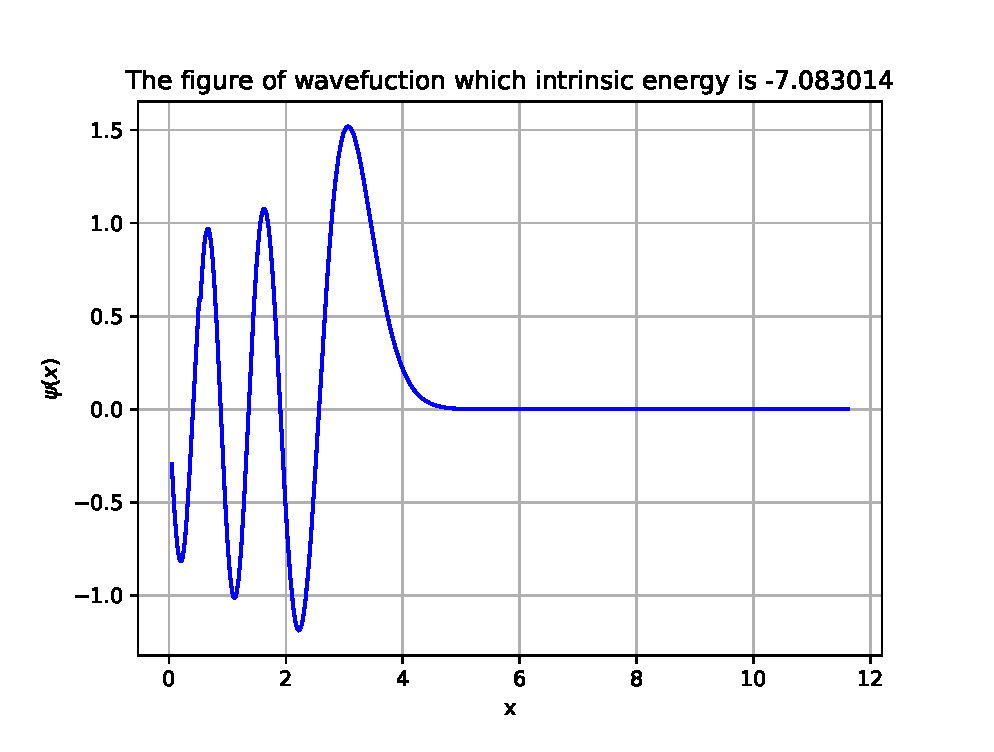
\includegraphics[width=0.9\linewidth]{figure/6}
	\label{fig:6}
\end{figure}
\begin{figure}
	\centering
	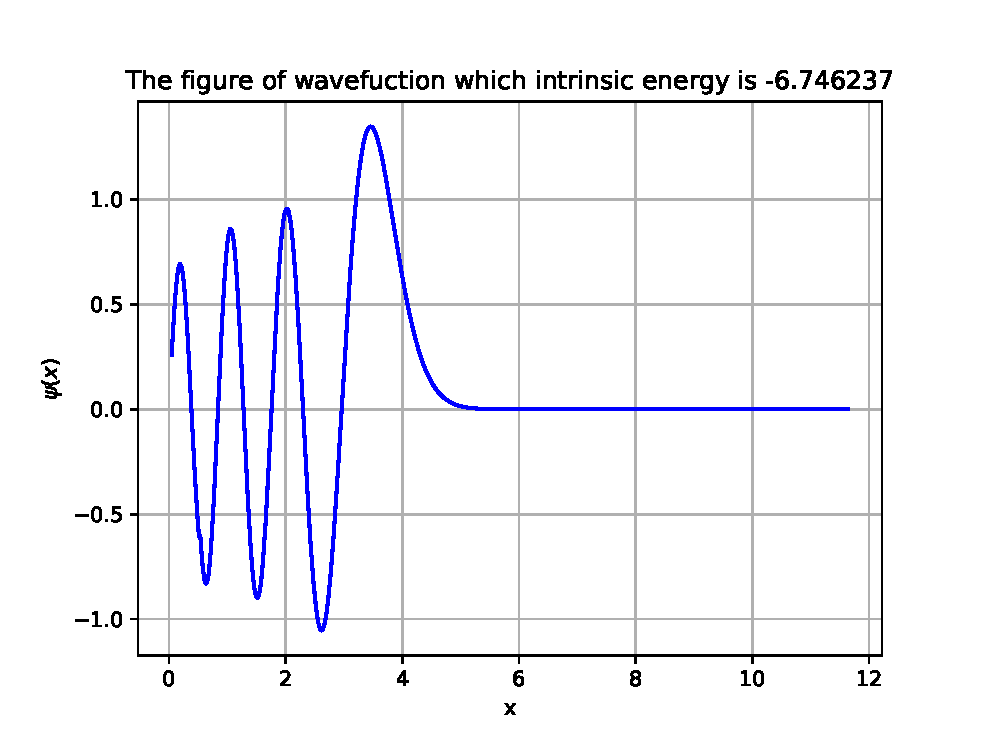
\includegraphics[width=0.9\linewidth]{figure/7}
	\label{fig:7}
\end{figure}
\begin{figure}
	\centering
	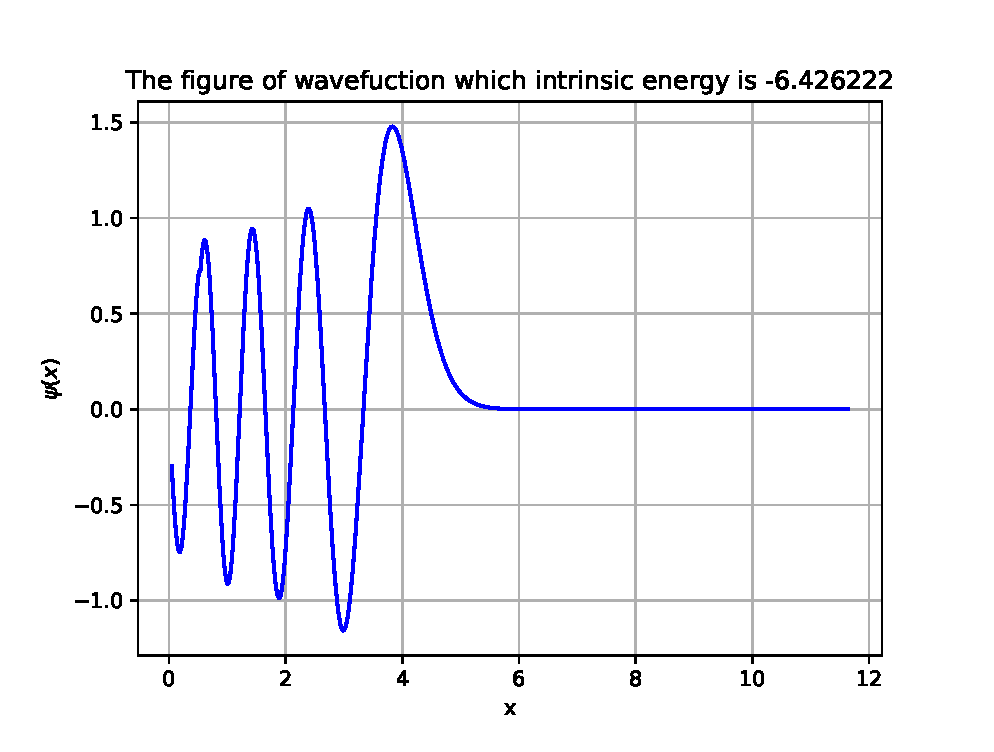
\includegraphics[width=0.9\linewidth]{figure/8}
	\label{fig:8}
\end{figure}
\begin{figure}
	\centering
	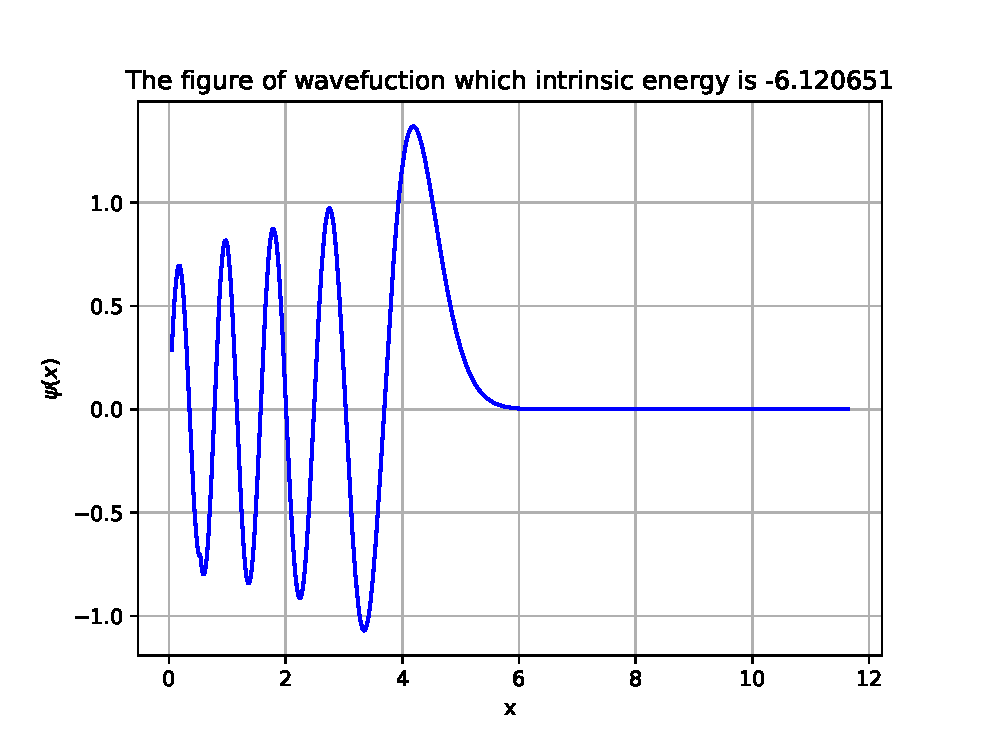
\includegraphics[width=0.9\linewidth]{figure/9}
	\label{fig:9}
\end{figure}
\begin{figure}
	\centering
	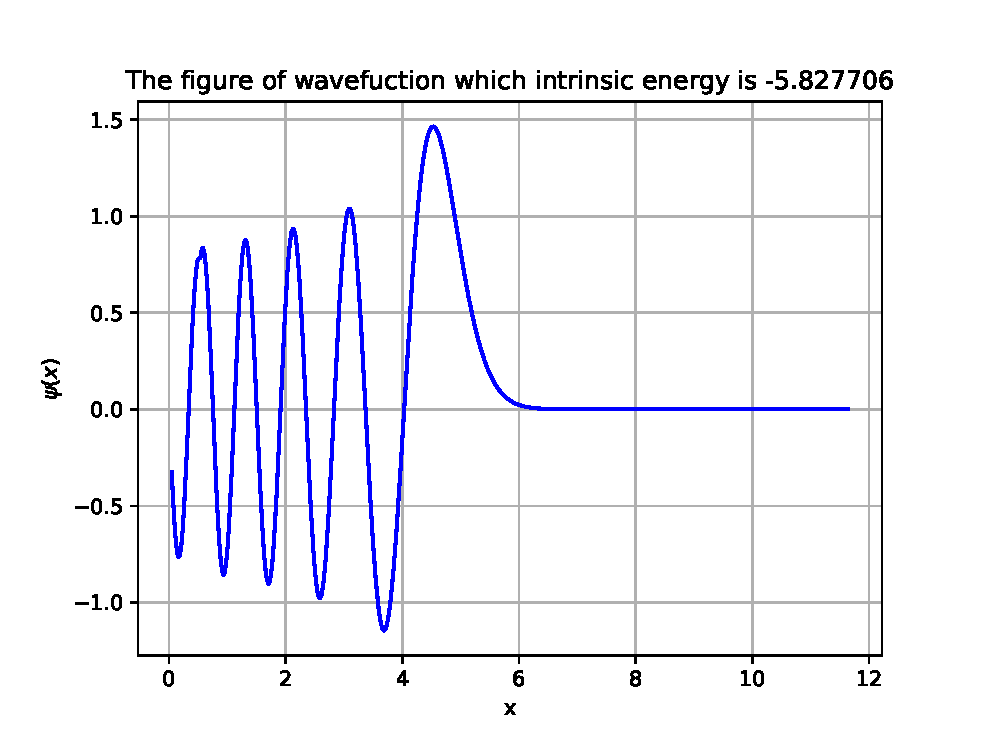
\includegraphics[width=0.9\linewidth]{figure/10}
	\label{fig:10}
\end{figure}
\begin{figure}
	\centering
	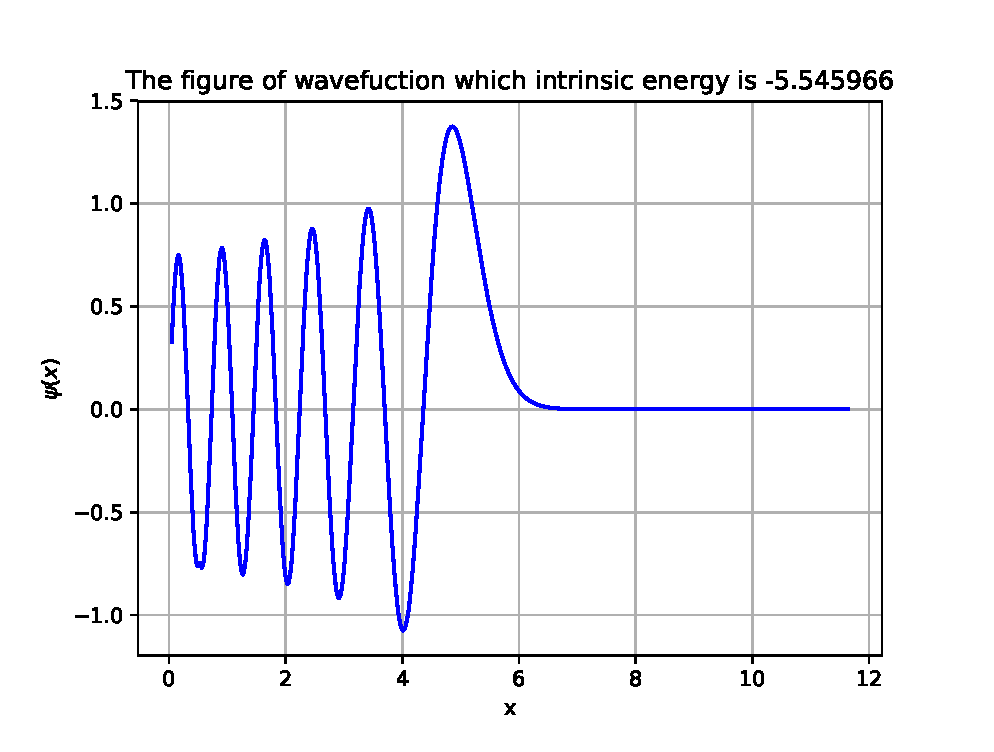
\includegraphics[width=0.9\linewidth]{figure/11}
	\label{fig:11}
\end{figure}
\begin{figure}
	\centering
	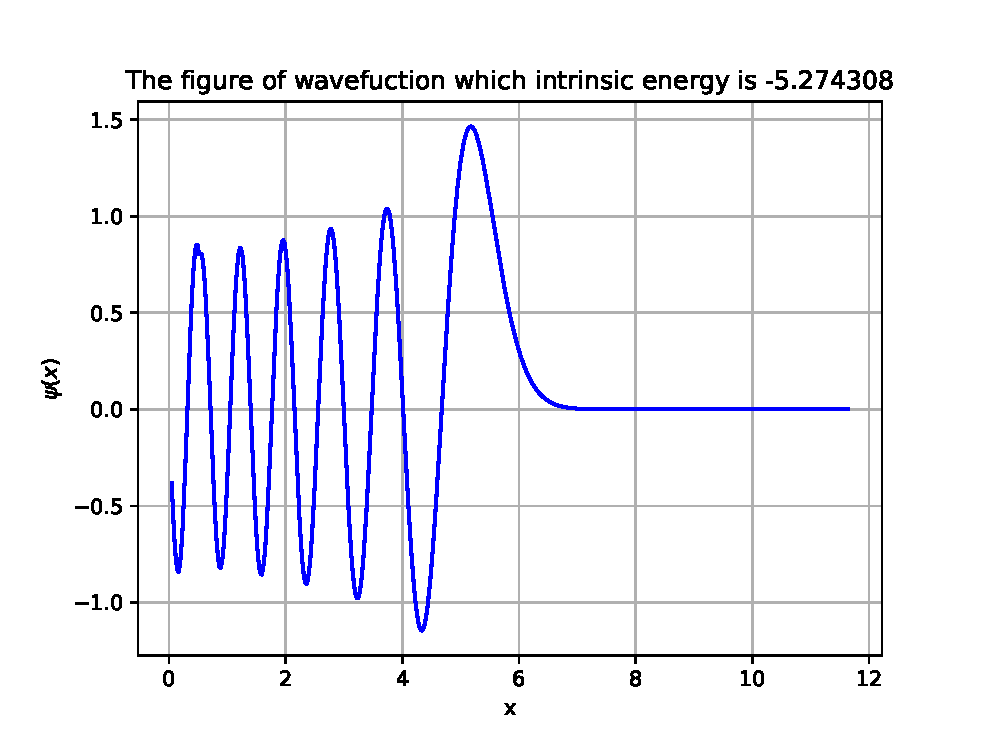
\includegraphics[width=0.9\linewidth]{figure/12}
	\label{fig:12}
\end{figure}
\begin{figure}
	\centering
	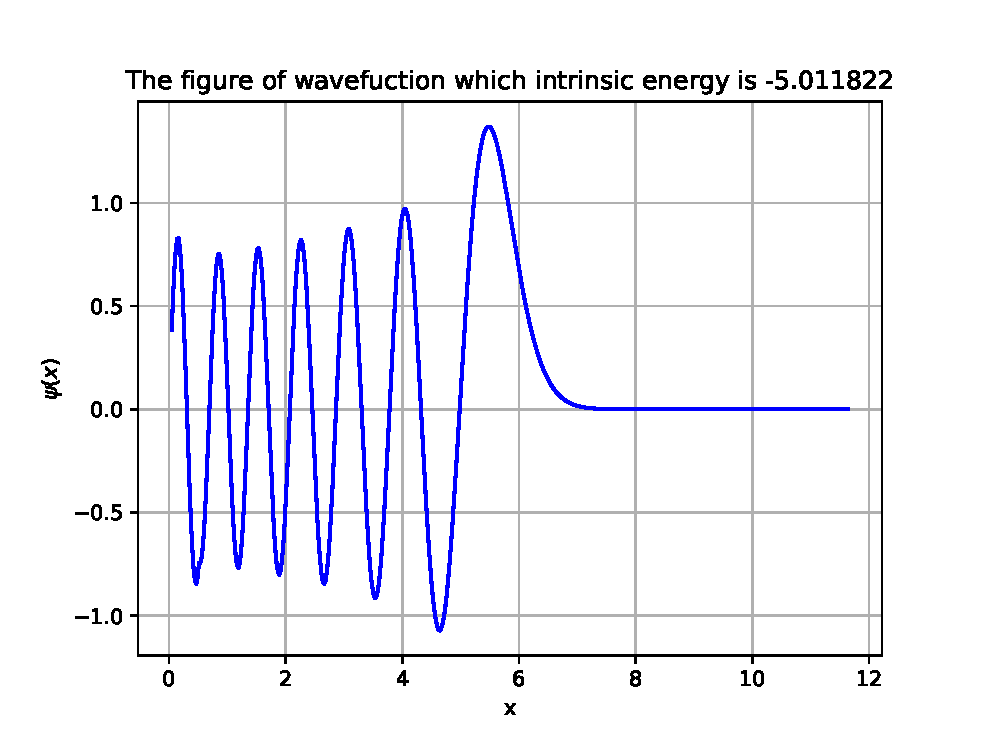
\includegraphics[width=0.9\linewidth]{figure/13}
	\label{fig:13}
\end{figure}
\begin{figure}
	\centering
	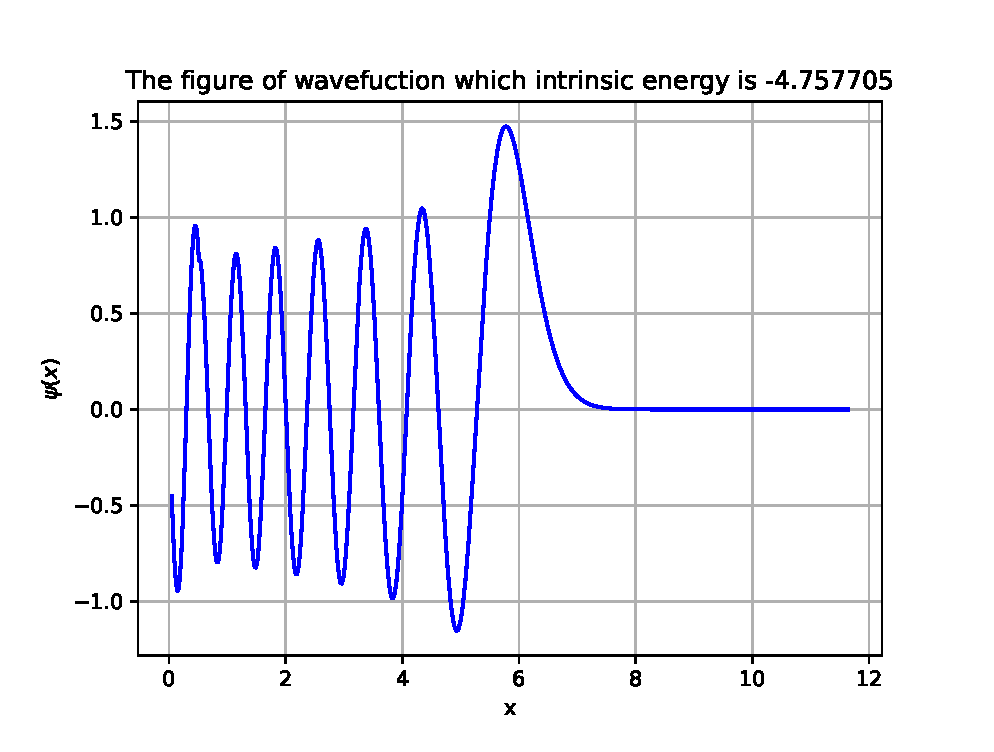
\includegraphics[width=0.9\linewidth]{figure/14}
	\label{fig:14}
\end{figure}
\begin{figure}
	\centering
	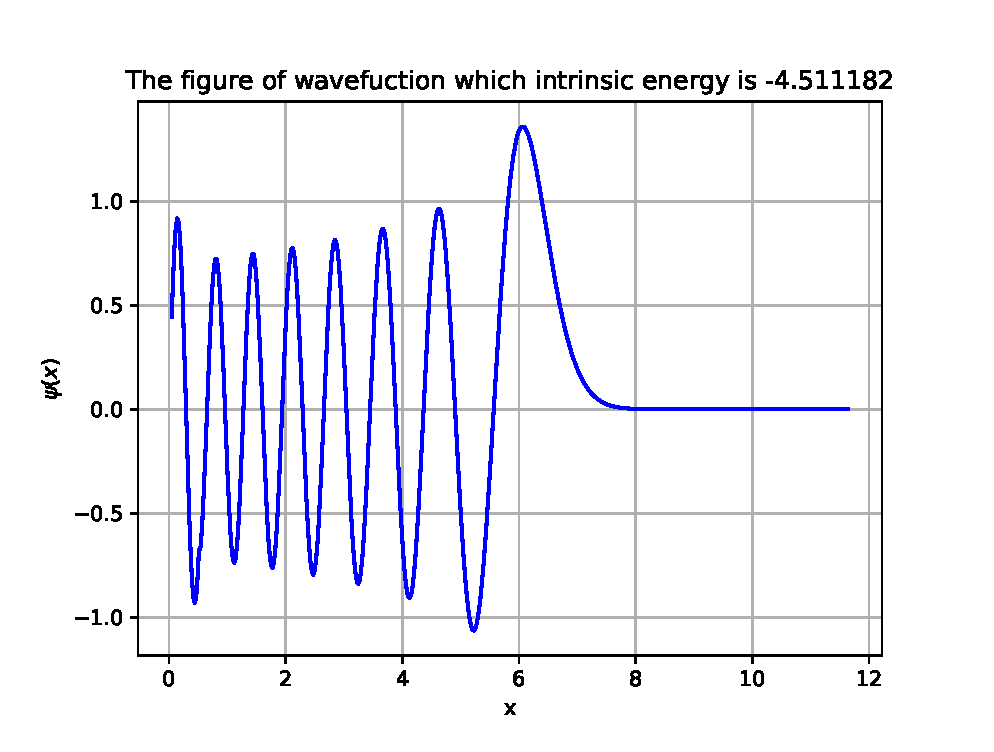
\includegraphics[width=0.9\linewidth]{figure/15}
	\label{fig:15}
\end{figure}
\begin{figure}
	\centering
	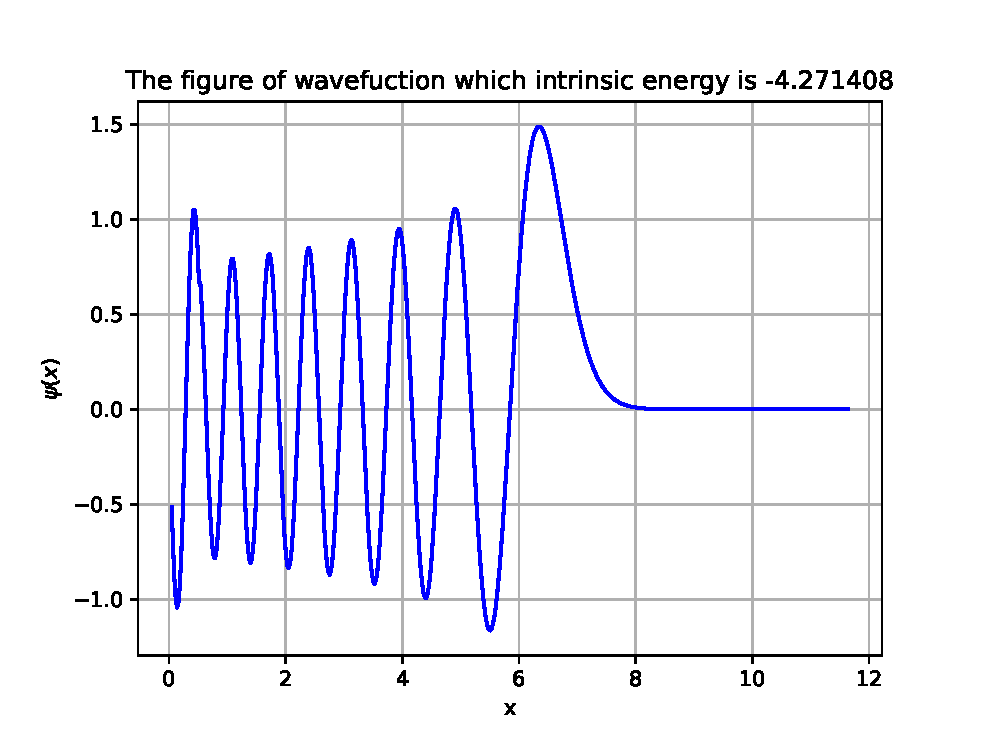
\includegraphics[width=0.9\linewidth]{figure/16}
	\label{fig:16}
\end{figure}
\begin{figure}
	\centering
	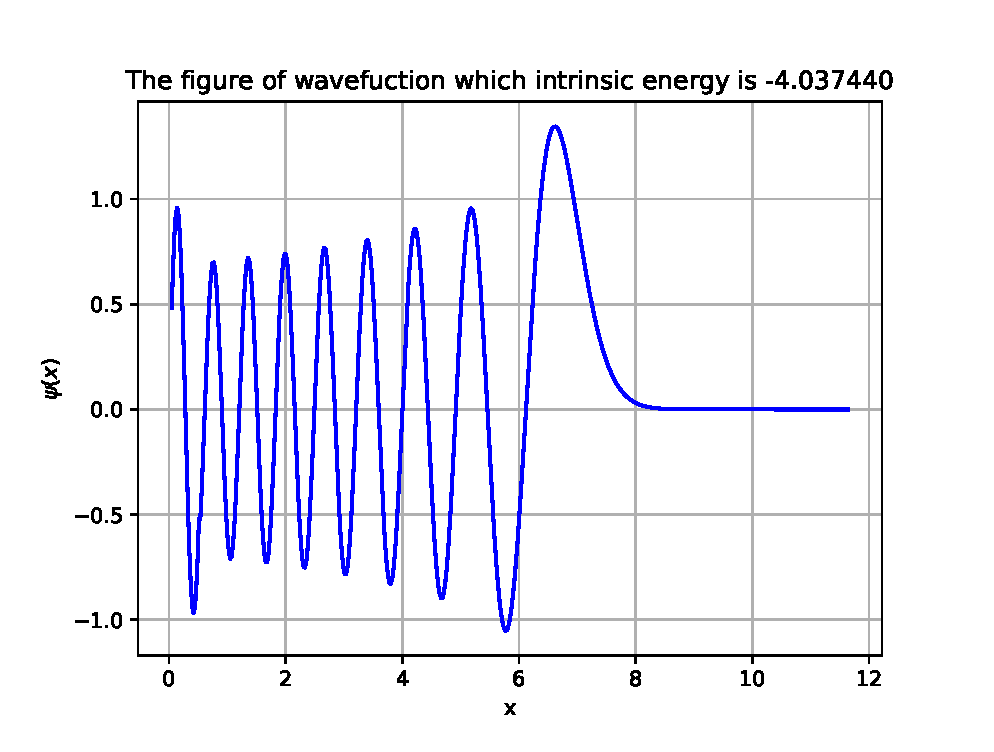
\includegraphics[width=0.9\linewidth]{figure/17}
	\label{fig:17}
\end{figure}
\begin{figure}
	\centering
	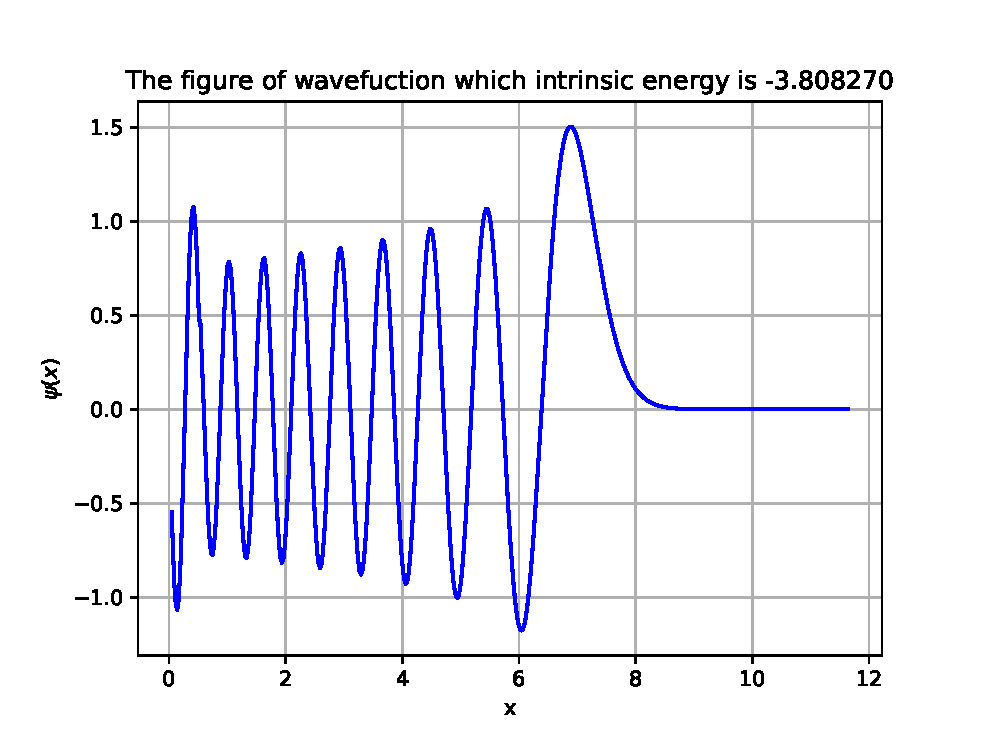
\includegraphics[width=0.9\linewidth]{figure/18}
	\label{fig:18}
\end{figure}
\begin{figure}
	\centering
	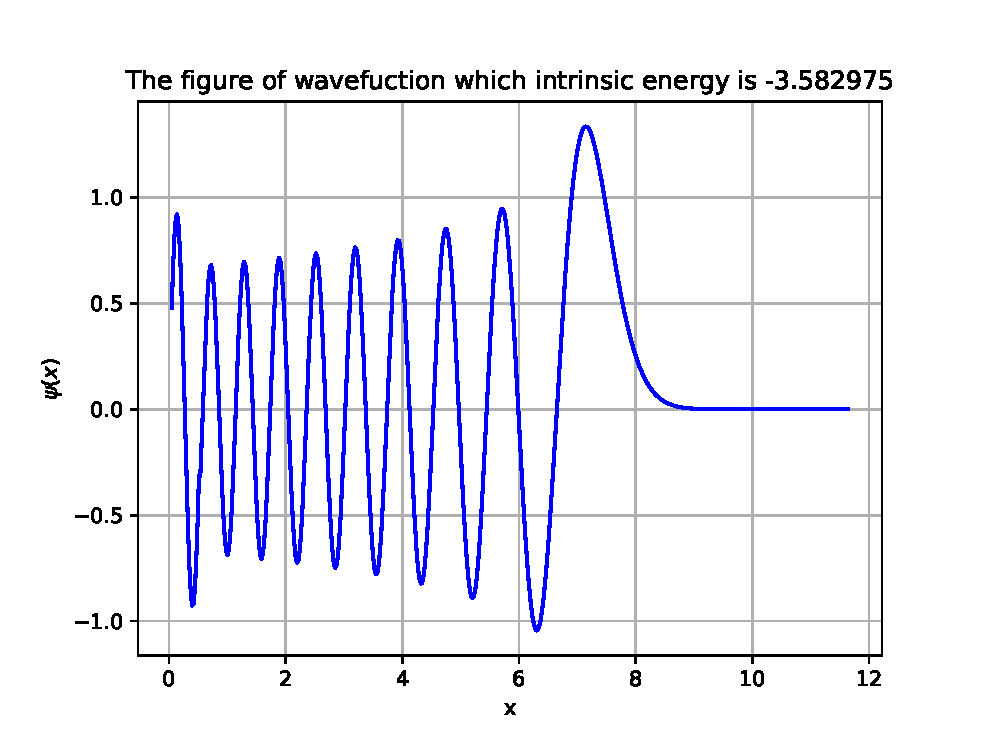
\includegraphics[width=0.9\linewidth]{figure/19}
	\label{fig:19}
\end{figure}
\begin{figure}
	\centering
	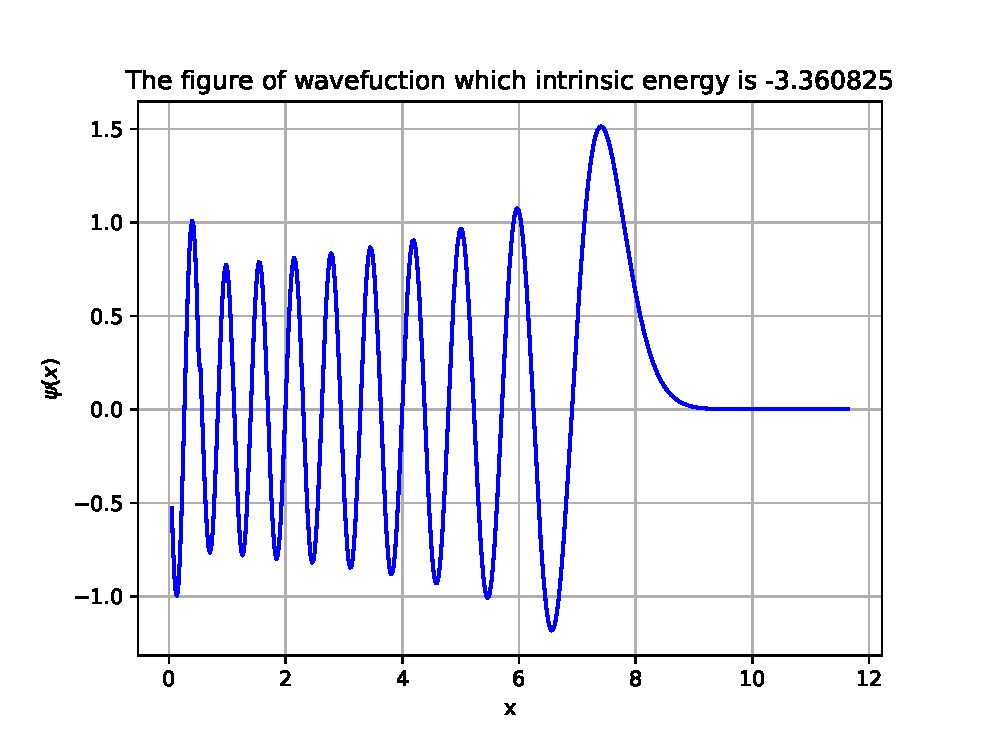
\includegraphics[width=0.9\linewidth]{figure/20}
	\label{fig:20}
\end{figure}
\begin{figure}
	\centering
	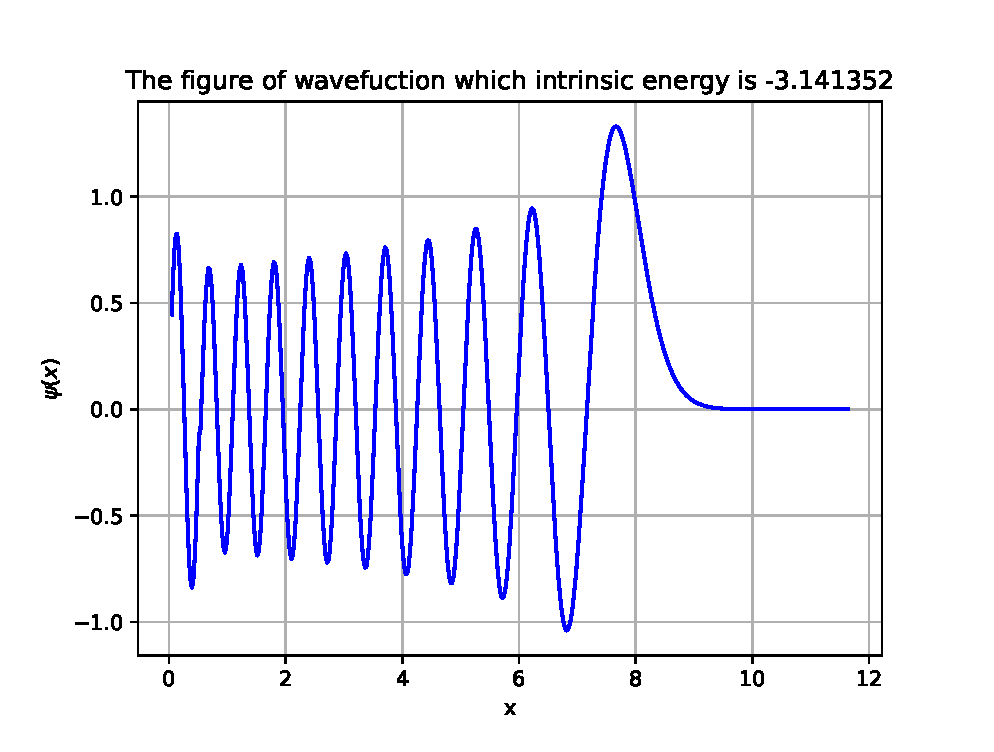
\includegraphics[width=0.9\linewidth]{figure/21}
	\label{fig:21}
\end{figure}
\begin{figure}
	\centering
	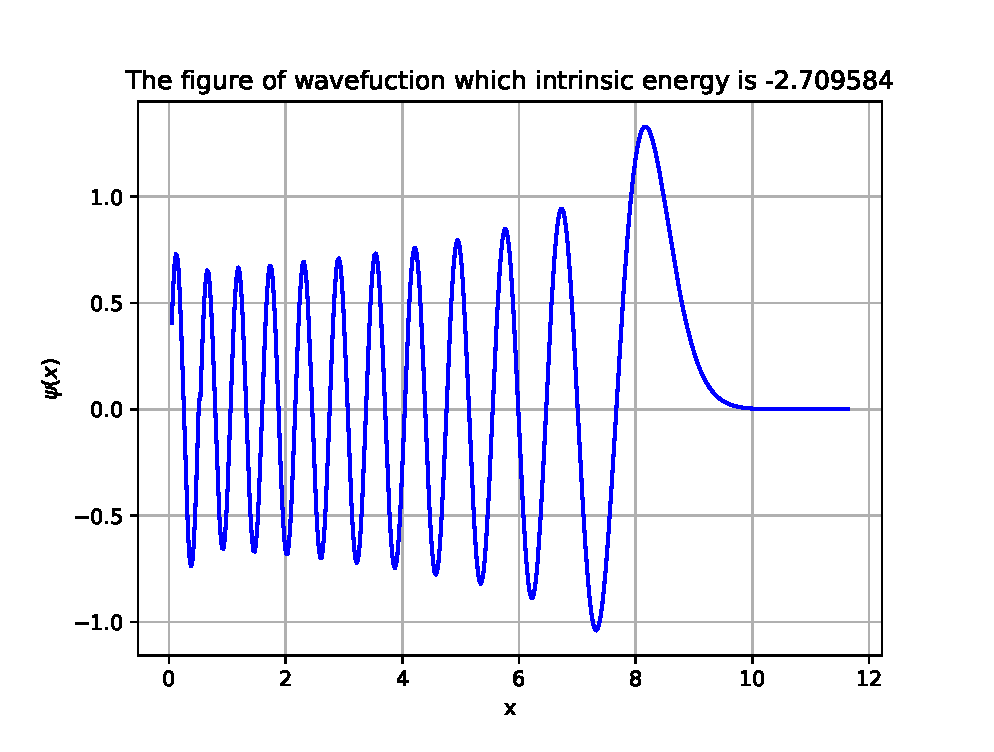
\includegraphics[width=0.9\linewidth]{figure/22}
	\label{fig:22}
\end{figure}
\begin{figure}
	\centering
	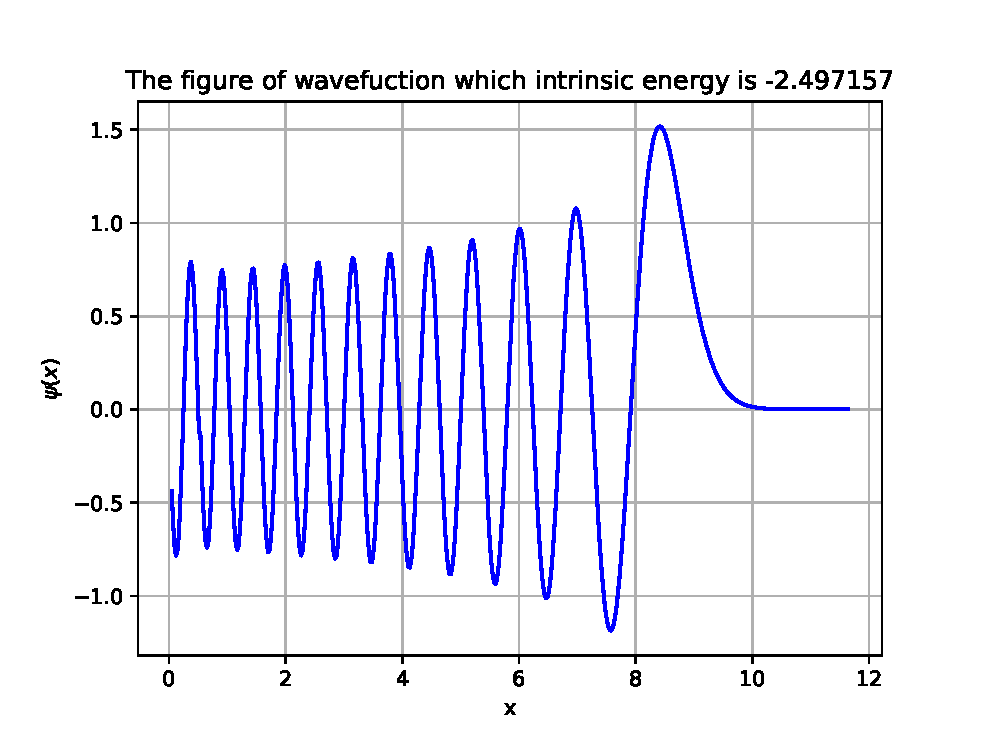
\includegraphics[width=0.9\linewidth]{figure/23}
	\label{fig:23}
\end{figure}
\begin{figure}
	\centering
	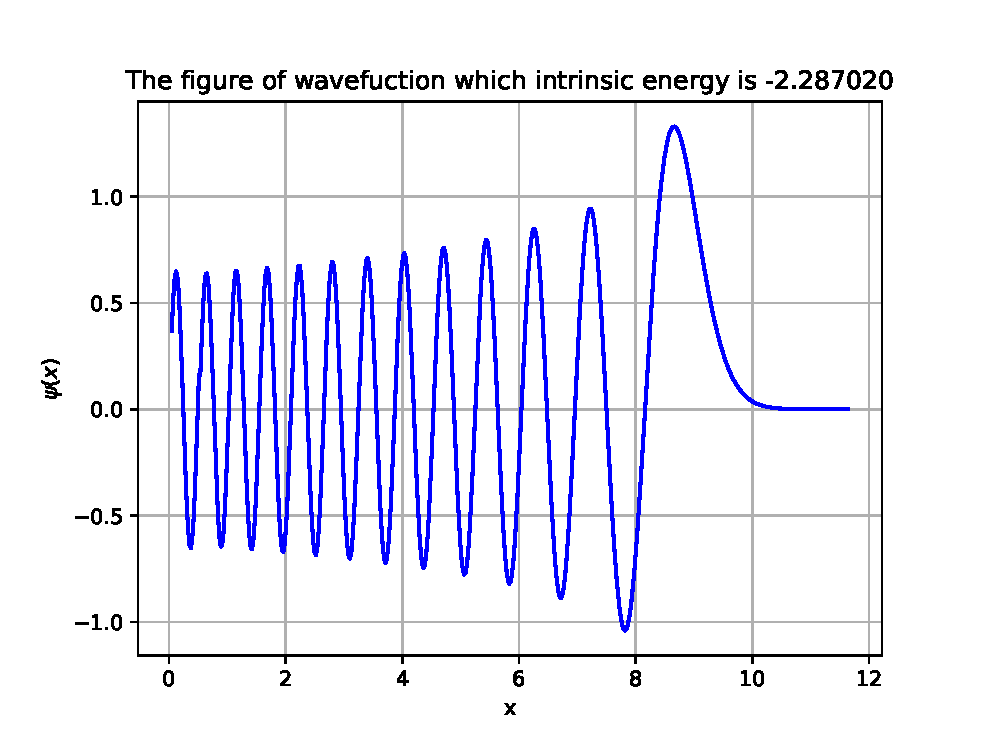
\includegraphics[width=0.9\linewidth]{figure/24}
	\label{fig:24}
\end{figure}
\begin{figure}
	\centering
	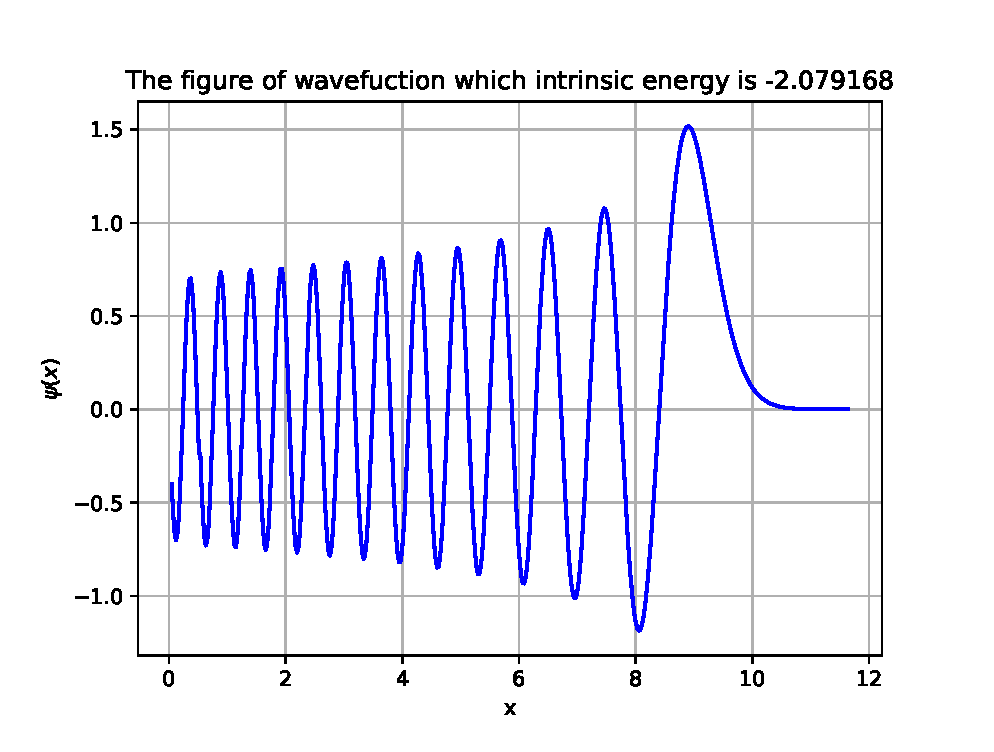
\includegraphics[width=0.9\linewidth]{figure/25}
	\label{fig:25}
\end{figure}
\begin{figure}
	\centering
	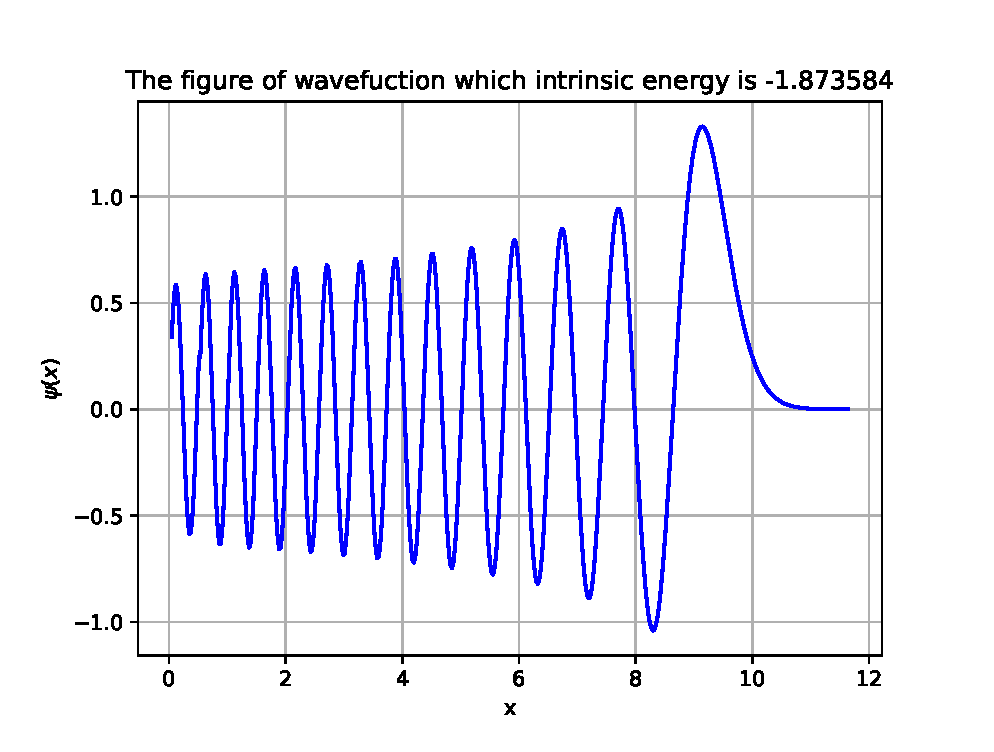
\includegraphics[width=0.9\linewidth]{figure/26}
	\label{fig:26}
\end{figure}
\begin{figure}
	\centering
	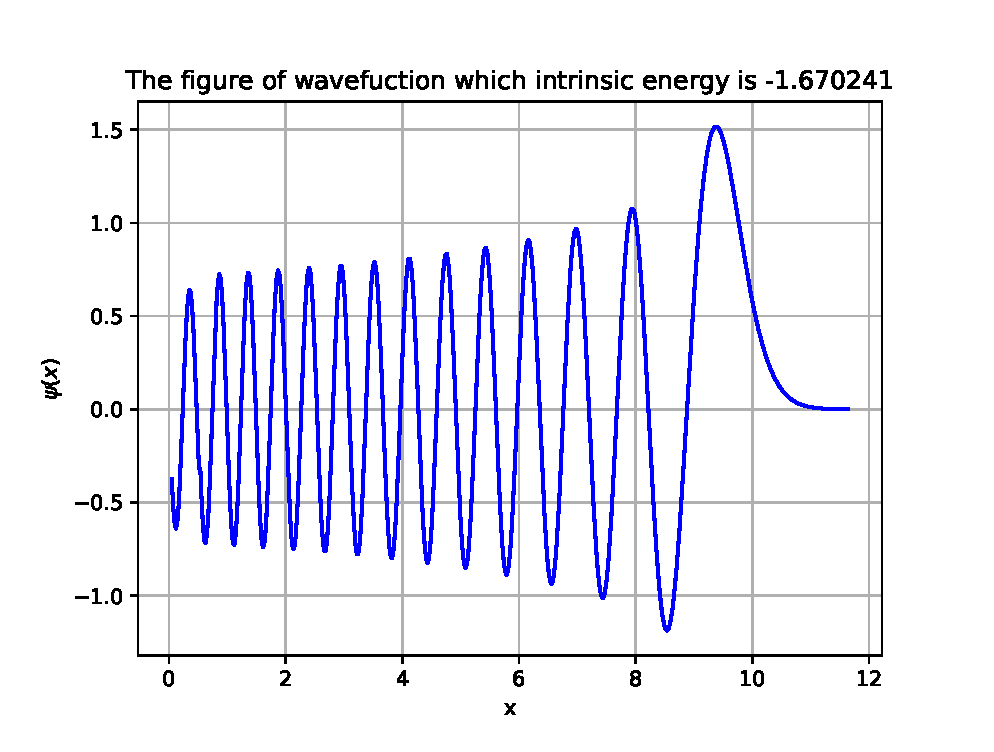
\includegraphics[width=0.9\linewidth]{figure/27}
	\label{fig:27}
\end{figure}
\begin{figure}
	\centering
	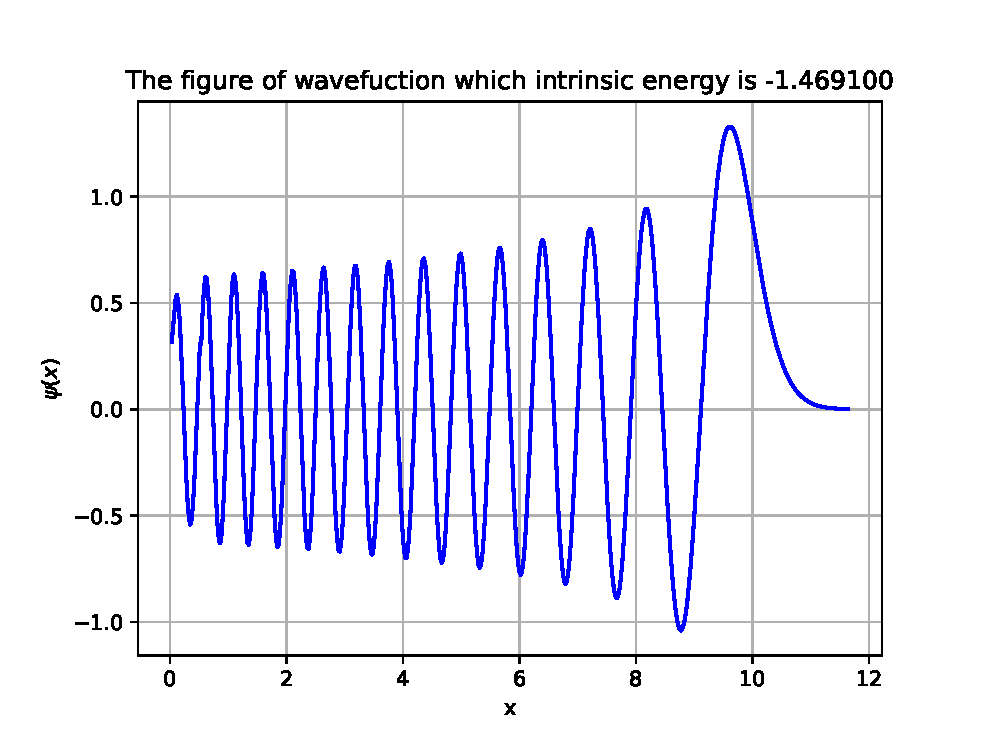
\includegraphics[width=0.9\linewidth]{figure/28}
	\label{fig:28}
\end{figure}
\begin{figure}
	\centering
	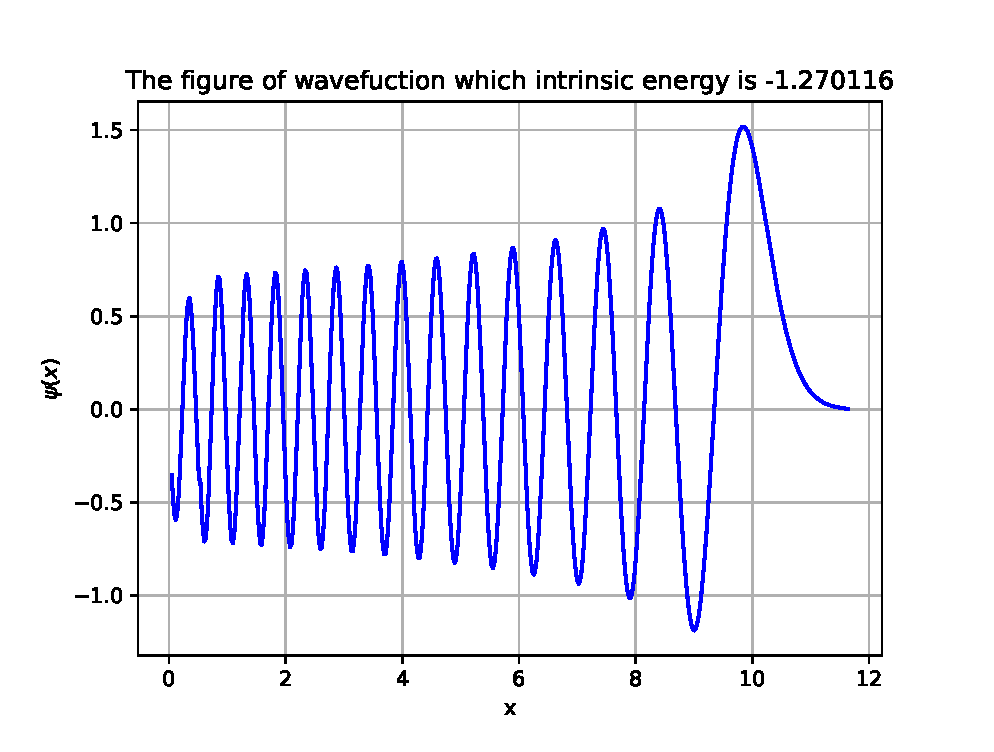
\includegraphics[width=0.9\linewidth]{figure/29}
	\label{fig:29}
\end{figure}
\begin{figure}
	\centering
	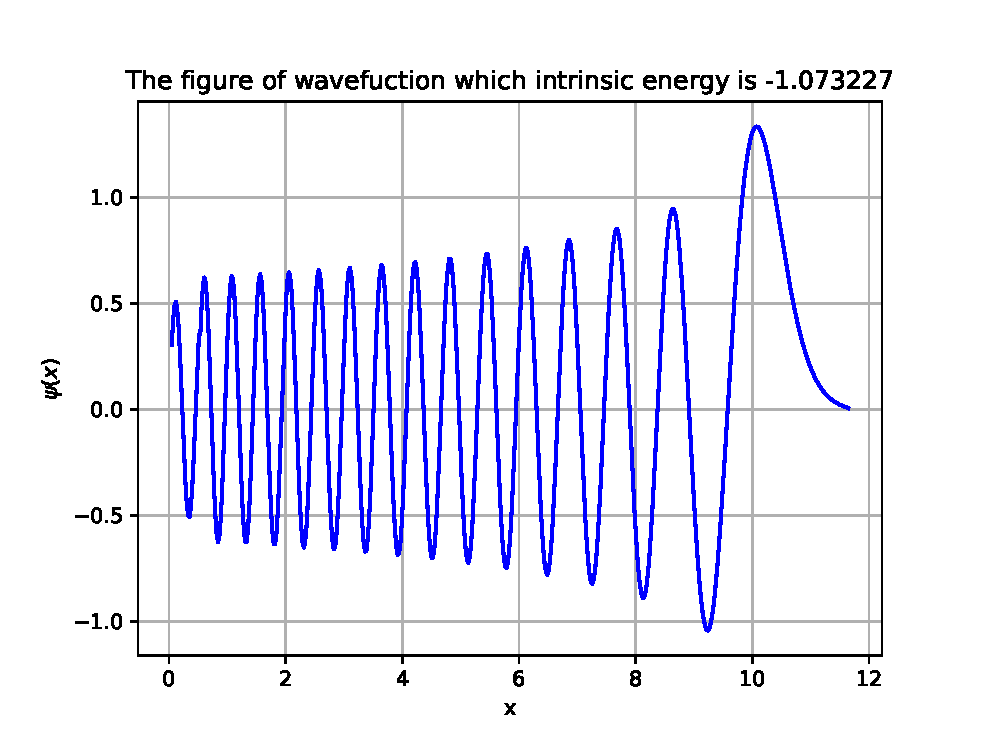
\includegraphics[width=0.9\linewidth]{figure/30}
	\label{fig:30}
\end{figure}
\begin{figure}
	\centering
	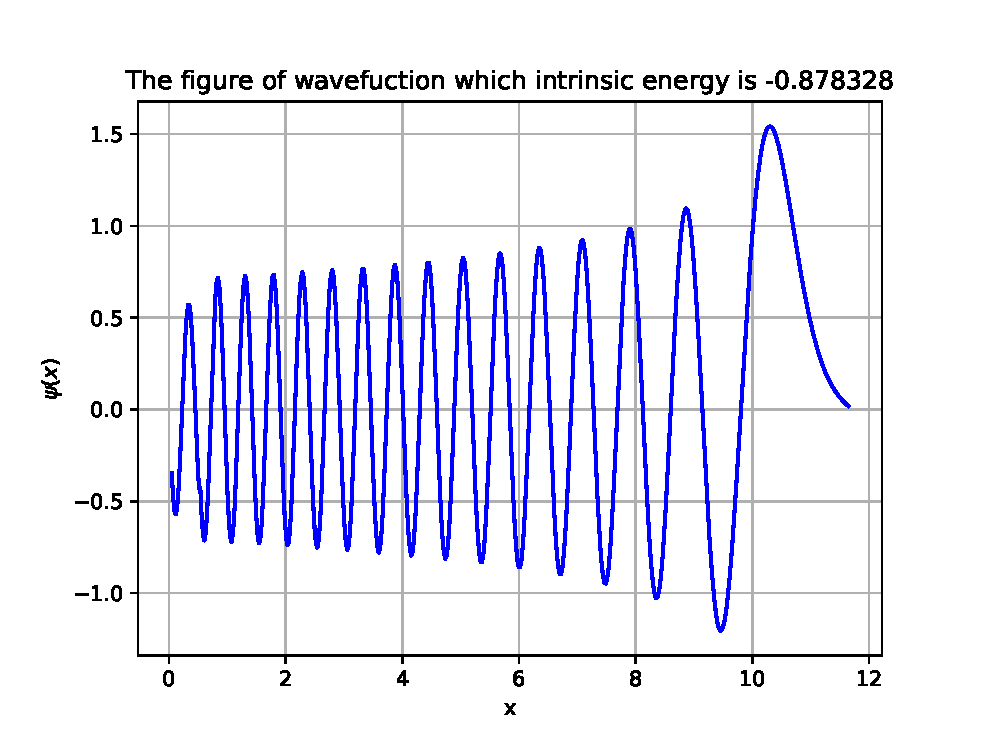
\includegraphics[width=0.9\linewidth]{figure/31}
	\label{fig:31}
\end{figure}
\begin{figure}
	\centering
	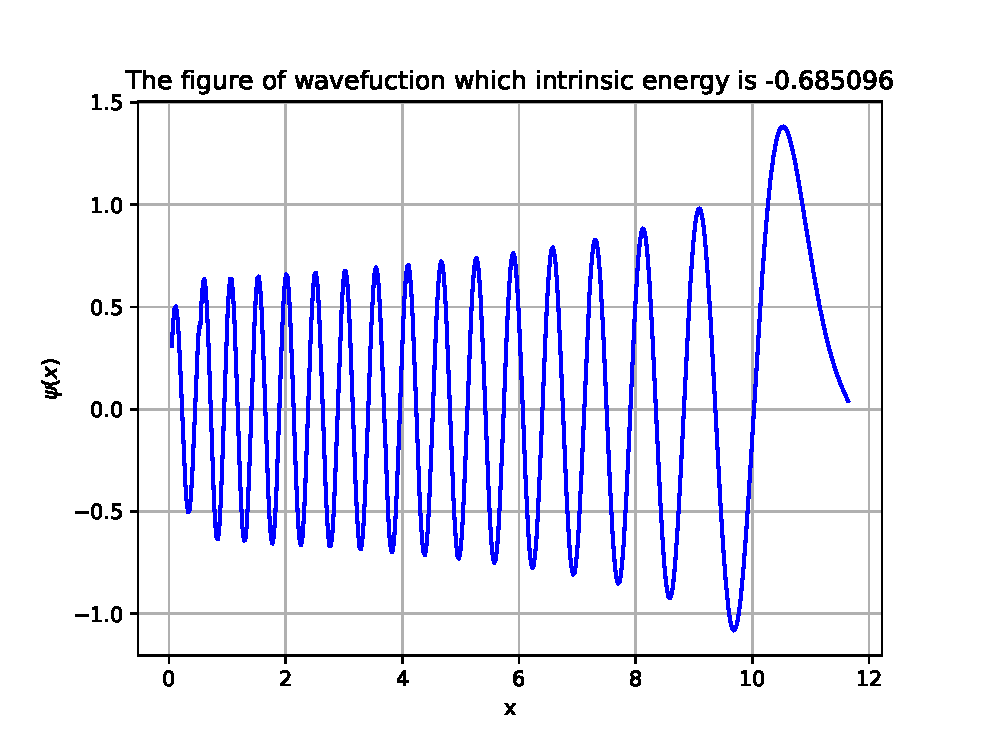
\includegraphics[width=0.9\linewidth]{figure/32}
	\label{fig:32}
\end{figure}
\begin{figure}
	\centering
	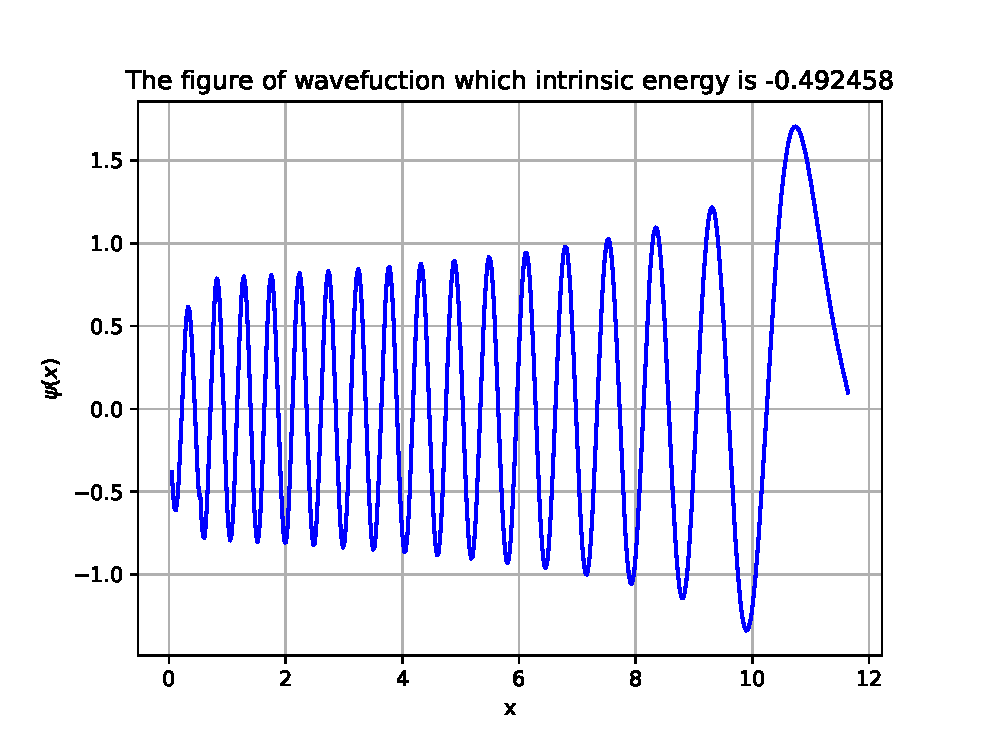
\includegraphics[width=0.9\linewidth]{figure/33}
	\label{fig:33}
\end{figure}
\begin{figure}
	\centering
	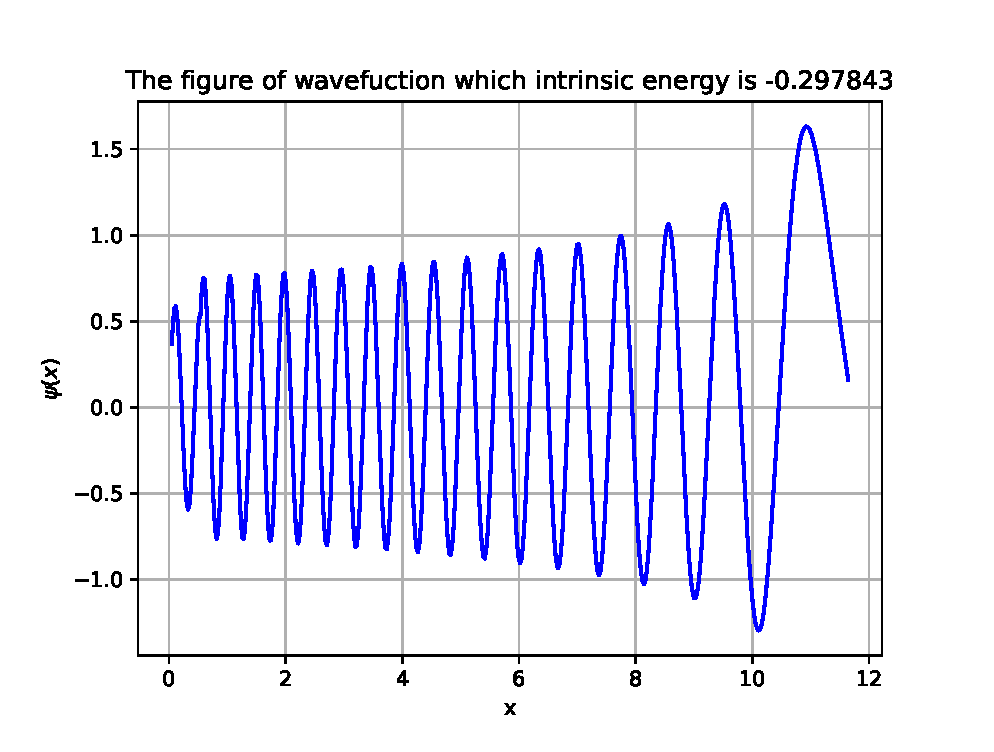
\includegraphics[width=0.9\linewidth]{figure/34}
	\label{fig:34}
\end{figure}
\begin{figure}
	\centering
	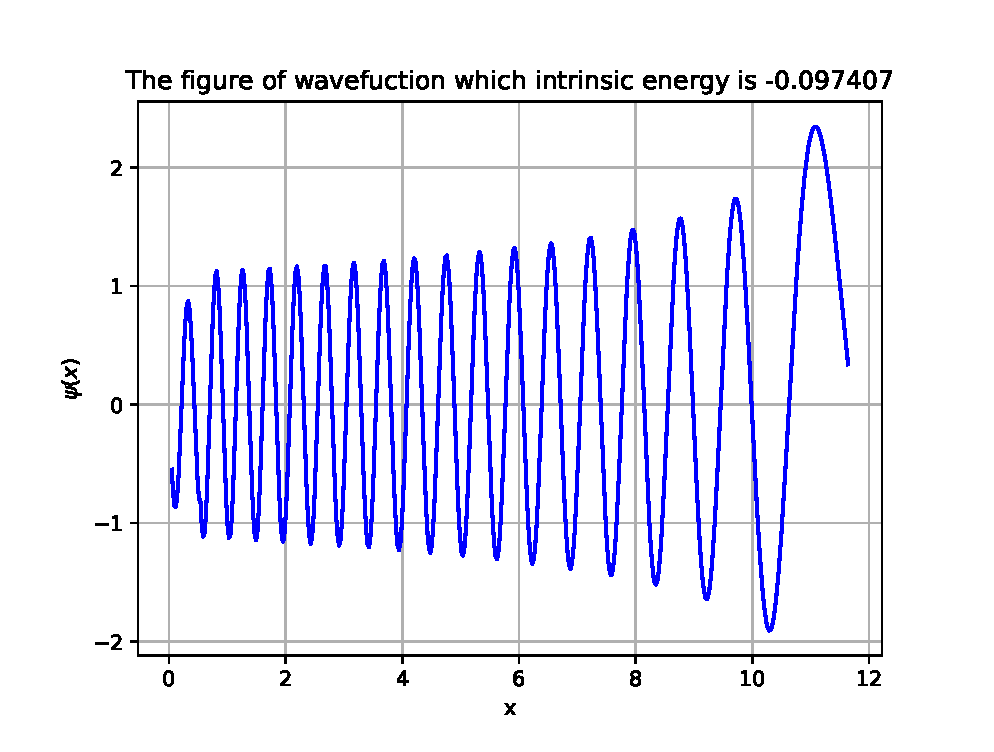
\includegraphics[width=0.9\linewidth]{figure/35}
	\label{fig:35}
\end{figure}
\begin{figure}
	\centering
	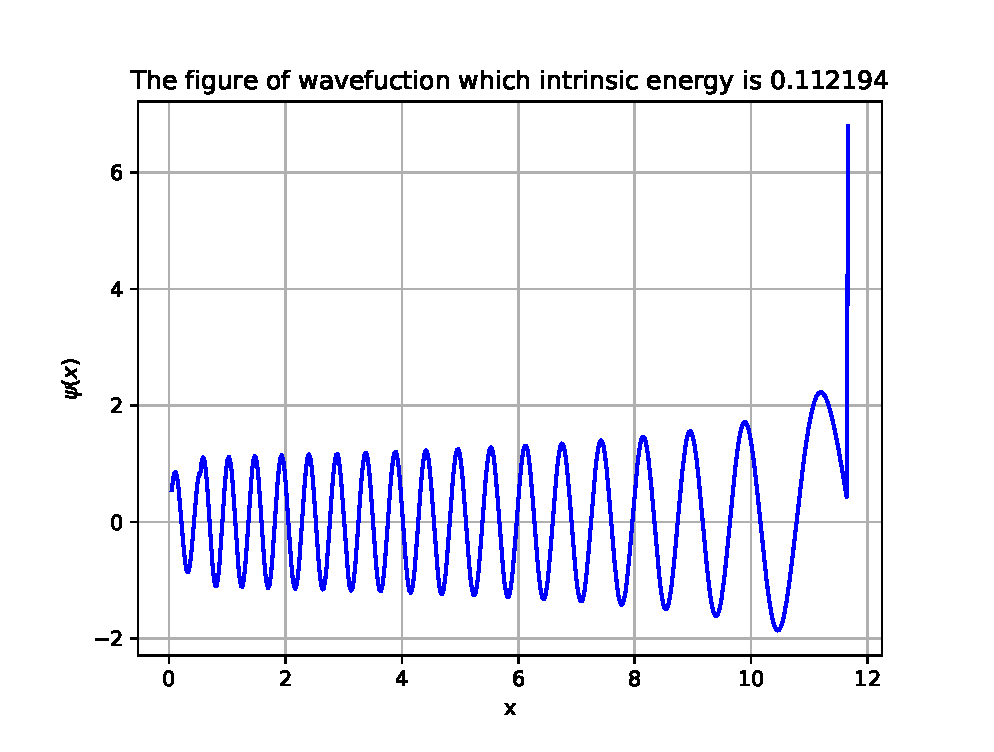
\includegraphics[width=0.9\linewidth]{figure/36}
	\label{fig:36}
\end{figure}

%----------------------------------------------------------------------------------------
%	APPENDICES SECTION
%----------------------------------------------------------------------------------------

\newpage
\onecolumn
\begin{appendices}
\section{计算求解部分}
这是运用打靶法求解schrodinger方程的C语言程序。\\
\textbf{\textcolor[rgb]{0.98,0.00,0.00}{Input C source:}}
\lstinputlisting[language=C]{./program/schrodinger.c}
\section{读数绘图部分}
这是运用Python直接读取Excel数据绘制波函数图像的程序。\\
\textbf{\textcolor[rgb]{0.98,0.00,0.00}{Input Python source:}}
\lstinputlisting[language=C]{./program/plot.py}
\end{appendices}

%----------------------------------------------------------------------------------------
%	REFERENCE
%----------------------------------------------------------------------------------------

\newpage
\renewcommand\refname{参考文献}
\begin{thebibliography}{99}
\bibitem{ref1}P. A. M. Dirac (1958). The Principles of Quantum Mechanics (4th ed.). Oxford University Press. ISBN 0-198-51208-2.
\bibitem{ref2}B.H. Bransden \& C.J. Joachain (2000). Quantum Mechanics (2nd ed.). Prentice Hall PTR. ISBN 0-582-35691-1.
\bibitem{ref3}David J. Griffiths (2004). Introduction to Quantum Mechanics (2nd ed.). Benjamin Cummings. ISBN 0-13-124405-1.
\bibitem{ref4}Hall, Brian C. (2013), Quantum Theory for Mathematicians, Graduate Texts in Mathematics, 267, Springer, ISBN 978-1461471158.
\bibitem{ref5}Richard Liboff (2002). Introductory Quantum Mechanics (4th ed.). Addison Wesley. ISBN 0-8053-8714-5.
\bibitem{ref6}Serway, Moses, and Moyer (2004). Modern Physics (3rd ed.). Brooks Cole. ISBN 0-534-49340-8.
\bibitem{ref7}Schrödinger, Erwin (December 1926). "An Undulatory Theory of the Mechanics of Atoms and Molecules". Phys. Rev. 28 (6): 1049–1070. Bibcode:1926PhRv...28.1049S. doi:10.1103/PhysRev.28.1049.
\bibitem{ref8}Teschl, Gerald (2009). Mathematical Methods in Quantum Mechanics; With Applications to Schrödinger Operators. Providence: American Mathematical Society. ISBN 978-0-8218-4660-5.
\bibitem{ref9}Numerov, Boris Vasil'evich (1924), "A method of extrapolation of perturbations", Monthly Notices of the Royal Astronomical Society, 84: 592–601, Bibcode:1924MNRAS..84..592N, doi:10.1093/mnras/84.8.592.
\bibitem{ref10}Numerov, Boris Vasil'evich (1927), "Note on the numerical integration of d2x/dt2 = f(x,t)", Astronomische Nachrichten, 230: 359–364, Bibcode:1927AN....230..359N, doi:10.1002/asna.19272301903.
\bibitem{ref11}J Killingbeck, Shooting methods for the Schrodinger equation, J. Phys. A: Math. Gen. 20 (1987) 1411-1417. Printed in the U.K.
\bibitem{ref12}https://zqyin.wordpress.com/2011/08/02/1dshrodinger/
\end{thebibliography} 

%----------------------------------------------------------------------------------------
\end{CJK*}
\end{document}
